\PassOptionsToPackage{unicode=true}{hyperref} % options for packages loaded elsewhere
\PassOptionsToPackage{hyphens}{url}
%
\documentclass[12pt,12pt,openright,oneside,a4paper,chapter=TITLE,section=TITLE,subsection=TITLE,subsubsection=TITLE english,french,spanish,portugues,sumario=tradicional]{abntex2}
\usepackage{lmodern}
\usepackage{amssymb,amsmath}
\usepackage{ifxetex,ifluatex}
\usepackage{fixltx2e} % provides \textsubscript
\ifnum 0\ifxetex 1\fi\ifluatex 1\fi=0 % if pdftex
  \usepackage[T1]{fontenc}
  \usepackage[utf8]{inputenc}
  \usepackage{textcomp} % provides euro and other symbols
\else % if luatex or xelatex
  \usepackage{unicode-math}
  \defaultfontfeatures{Ligatures=TeX,Scale=MatchLowercase}
\fi
% use upquote if available, for straight quotes in verbatim environments
\IfFileExists{upquote.sty}{\usepackage{upquote}}{}
% use microtype if available
\IfFileExists{microtype.sty}{%
\usepackage[]{microtype}
\UseMicrotypeSet[protrusion]{basicmath} % disable protrusion for tt fonts
}{}
\IfFileExists{parskip.sty}{%
\usepackage{parskip}
}{% else
\setlength{\parindent}{0pt}
\setlength{\parskip}{6pt plus 2pt minus 1pt}
}
\usepackage{hyperref}
\hypersetup{
            pdfauthor={Jackson da Silva Torres},
            pdfborder={0 0 0},
            breaklinks=true}
\urlstyle{same}  % don't use monospace font for urls
\usepackage{longtable,booktabs}
% Fix footnotes in tables (requires footnote package)
\IfFileExists{footnote.sty}{\usepackage{footnote}\makesavenoteenv{longtable}}{}
\usepackage{graphicx,grffile}
\makeatletter
\def\maxwidth{\ifdim\Gin@nat@width>\linewidth\linewidth\else\Gin@nat@width\fi}
\def\maxheight{\ifdim\Gin@nat@height>\textheight\textheight\else\Gin@nat@height\fi}
\makeatother
% Scale images if necessary, so that they will not overflow the page
% margins by default, and it is still possible to overwrite the defaults
% using explicit options in \includegraphics[width, height, ...]{}
\setkeys{Gin}{width=\maxwidth,height=\maxheight,keepaspectratio}
\setlength{\emergencystretch}{3em}  % prevent overfull lines
\providecommand{\tightlist}{%
  \setlength{\itemsep}{0pt}\setlength{\parskip}{0pt}}
\setcounter{secnumdepth}{5}
% Redefines (sub)paragraphs to behave more like sections
\ifx\paragraph\undefined\else
\let\oldparagraph\paragraph
\renewcommand{\paragraph}[1]{\oldparagraph{#1}\mbox{}}
\fi
\ifx\subparagraph\undefined\else
\let\oldsubparagraph\subparagraph
\renewcommand{\subparagraph}[1]{\oldsubparagraph{#1}\mbox{}}
\fi

% set default figure placement to htbp
\makeatletter
\def\fps@figure{htbp}
\makeatother

%%%%%%%%%%%%%%%%%%%%%%%%%%%%%%%%%%%%%%%%%%%%%%%%%%%%%%%
% Arquivo para entrada de dados para a parte pré textual
%%%%%%%%%%%%%%%%%%%%%%%%%%%%%%%%%%%%%%%%%%%%%%%%%%%%%%%
% 
% Basta digitar as informações indicidas, no formato 
% apresentado.
%
%%%%%%%
% Os dados solicitados são, na ordem:
%
% tipo do trabalho
% componentes do trabalho 
% título do trabalho
% nome do autor
% local 
% data (ano com 4 dígitos)
% orientador(a)
% coorientador(a)(as)(es)
% arquivo com dados bibliográficos
% instituição
% setor
% programa de pós gradução
% curso
% preambulo
% data defesa
% CDU
% errata
% assinaturas - termo de aprovação
% resumos & palavras chave
% agradecimentos
% dedicatoria
% epígrafe


% Informações de dados para CAPA e FOLHA DE ROSTO
%----------------------------------------------------------------------------- 
\tipotrabalho{Dissertação}

% Marcar Sim para as partes que irão compor o documento pdf
%----------------------------------------------------------------------------- 
 \providecommand{\terCapa}{Sim}
 \providecommand{\terFolhaRosto}{Sim}
 \providecommand{\terTermoAprovacao}{Nao}
 \providecommand{\terDedicatoria}{Nao}
 \providecommand{\terFichaCatalografica}{Nao}
 \providecommand{\terEpigrafe}{Nao}
 \providecommand{\terAgradecimentos}{Nao}
 \providecommand{\terErrata}{Nao}
 \providecommand{\terListaFiguras}{Sim}
 \providecommand{\terListaTabelas}{Sim}
 \providecommand{\terSiglasAbrev}{Nao}
 \providecommand{\terResumos}{Nao}
 \providecommand{\terSumario}{Sim}
 \providecommand{\terAnexo}{Nao}
 \providecommand{\terApendice}{Nao}
 \providecommand{\terIndiceR}{Nao}
%----------------------------------------------------------------------------- 

\titulo{Efeitos das variações dos componentes do \emph{Spread} na rentabilidade das instituições bancárias através da análise de dados em painel
}
\autor{}
\local{Curitiba}
\data{2020} %Apenas ano 4 dígitos

% Orientador ou Orientadora
\orientador{}
%Prof Emílio Eiji Kavamura, MSc}
\orientadora{
Prof\textordfeminine~Dra. Mayla Costa}
% Pode haver apenas uma orientadora ou um orientador
% Se houver os dois prevalece o feminino.

% Em termos de coorientação, podem haver até quatro neste modelo
% Sendo 2 mulhere e 2 homens.
% Coorientador ou Coorientadora
\coorientador{}%Prof Morgan Freeman, DSc}
\coorientadora{}

% Segundo Coorientador ou Segunda Coorientadora
\scoorientador{}
%Prof Jack Nicholson, DEng}
\scoorientadora{}
%Prof\textordfeminine~Ingrid Bergman, DEng}
% ----------------------------------------------------------
%\addbibresource{10-references/referencias.bib}
%\bibliography{10-references/referencias.bib}
% ----------------------------------------------------------
\instituicao{Universidade Federal do Paraná}

\def \ImprimirSetor{Departamento de Economia}%
%Setor de Tecnologia}

\def \ImprimirProgramaPos{Programa Profissional de Pós-Graduação em Economia}

\def \ImprimirCurso{Mestrado Profissional em Economia}

\preambulo{
Trabalho apresentado como requisito parcial para a obtenção do título de Mestre Profisisonal em Economia no curso de Mestrado Profissional em Economia pelo Departamento de Economia da Universidade Federal do Paraná}
%do grau de Bacharel em Expressão Gráfica no curso de Expressão Gráfica, Setor de Exatas da Universidade Federal do Paraná}

%----------------------------------------------------------------------------- 

\newcommand{\imprimirCurso}{}
%Programa de P\'os Gradua\c{c}\~ao em Engenharia da Constru\c{c}\~ao Civil}

\newcommand{\imprimirDataDefesa}{
31 de Dezembro de 2020}

\newcommand{\imprimircdu}{
02:141:005.7}

% ----------------------------------------------------------
\newcommand{\imprimirerrata}{

\vspace{\onelineskip}


\begin{table}[htb]
\center
\footnotesize
\begin{tabular}{|p{1.4cm}|p{1cm}|p{3cm}|p{3cm}|}
  \hline
   \textbf{Folha} & \textbf{Linha}  & \textbf{Onde se lê}  & \textbf{Leia-se}  \\
    \hline
    1 & 10 & auto-conclavo & autoconclavo\\
   \hline
\end{tabular}
\end{table}}

% Comandos de dados - Data da apresentação
\providecommand{\imprimirdataapresentacaoRotulo}{}
\providecommand{\imprimirdataapresentacao}{}
\newcommand{\dataapresentacao}[2][\dataapresentacaoname]{\renewcommand{\dataapresentacao}{#2}}

% Comandos de dados - Nome do Curso
\providecommand{\imprimirnomedocursoRotulo}{}
\providecommand{\imprimirnomedocurso}{}
\newcommand{\nomedocurso}[2][\nomedocursoname]
  {\renewcommand{\imprimirnomedocursoRotulo}{#1}
\renewcommand{\imprimirnomedocurso}{#2}}


% ----------------------------------------------------------
\newcommand{\AssinaAprovacao}{

\assinatura{%\textbf
   {Professora} \\ UFPR}
   \assinatura{%\textbf
   {Professora} \\ ENSEADE}
   \assinatura{%\textbf
   {Professora} \\ TIT}
   %\assinatura{%\textbf{Professor} \\ Convidado 4}
      
   \begin{center}
    \vspace*{0.5cm}
    %{\large\imprimirlocal}
    %\par
    %{\large\imprimirdata}
    \imprimirlocal, \imprimirDataDefesa.
    \vspace*{1cm}
  \end{center}
  }
  
% ----------------------------------------------------------
%\newcommand{\Errata}{%\color{blue}
%Elemento opcional da \textcite[4.2.1.2]{NBR14724:2011}. Exemplo:
%}

% ----------------------------------------------------------
\newcommand{\EpigrafeTexto}{%\color{blue}
\textit{Texto}
}

% ----------------------------------------------------------
\newcommand{\ResumoTexto}{%\color{blue}

}

\newcommand{\PalavraschaveTexto}{%\color{blue}
latex. abntex. editoração de texto.}

% ----------------------------------------------------------
\newcommand{\AbstractTexto}{%\color{blue}
This is the english abstract.
}
% ---
\newcommand{\KeywordsTexto}{%\color{blue}
latex. abntex. text editoration.
}

% ----------------------------------------------------------
\newcommand{\Resume}
{%\color{blue}
Il s'agit d'un résumé en français.
} 
% ---
\newcommand{\Motscles}
{%\color{blue}
 latex. abntex. publication de textes.
}

% ----------------------------------------------------------
\newcommand{\Resumen}
{%\color{blue}
Este es el resumen en español.
}
% ---
\newcommand{\Palabrasclave}
{%\color{blue}
latex. abntex. publicación de textos.
}

% ----------------------------------------------------------
\newcommand{\AgradecimentosTexto}{%\color{blue}

}

% ----------------------------------------------------------
\newcommand{\DedicatoriaTexto}{%\color{blue}
\textit{}
	}


%\usepackage{geometry}


% Pacotes básicos 
% ----------------------------------------------------------
%\usepackage{lmodern}			% Usa a fonte Latin Modern			
\usepackage[utf8]{inputenc}		% Codificacao do documento (conversão automática dos acentos)
\usepackage{csquotes}
\usepackage[T1]{fontenc}		% Selecao de codigos de fonte.
\usepackage{lastpage}			% Usado pela Ficha catalográfica
\usepackage{indentfirst}		% Indenta o primeiro parágrafo de cada seção.
\usepackage{color}		    	% Controle das cores
\usepackage{graphicx}			% Inclusão de gráficos
\usepackage{microtype} 			% para melhorias de justificação
\usepackage{ifthen}		    	% para montar condicionais
%\usepackage[brazil]{babel}		% para utilizar termos em portugues
\usepackage[final]{pdfpages}    % para incluir páginas de arquivos pdf
\usepackage{lipsum}				% para geração de dummy text
\usepackage{csquotes}

%\usepackage[style=long]{glossaries}
%\usepackage{abntex2glossaries}

% permite representar o cancelamento de termos em texto ou equacoes
\usepackage{cancel} 		
% cores extendidas
\usepackage{xcolor} 		
% gera diagramas a partir de listas
\usepackage{smartdiagram}   
% Para a figura ficar na posição correta
\usepackage{float} 		    
% supporte para fontes da Text Companion 
\usepackage{textcomp} 		
% uso de longtable
\usepackage{longtable}		
% simbolos matematicos
\usepackage{amsmath}	
% páginas em paisagem
\usepackage{lscape}
% mescla de colunas em tabelas
\usepackage{multicol}
% mescla de linhas em tabelas
\usepackage{multirow}
% criação do indice de quadros
\usepackage{newfloat} 
% configura legenda 
\usepackage{caption} 		
%[format=plain]
	%\renewcommand\caption[1]{%
    \captionsetup{font=small}	% tamanho da fonte 10pt
    %,format=hang
 	% \caption{#1}}
	%\captionsetup{width=0.8\textwidth}
	
%\usepackage{scrpage2}

% Pacotes de citações BibLaTeX
% ----------------------------------------------------------
\usepackage[
style=abnt,
%backref=true,
backend=biber,
maxcitenames=3,
%citecounter=true,
%backrefstyle=three,
nohashothers=true
]{biblatex}


\DefineBibliographyStrings{brazil}{%
 backrefpage = {Citado \arabic{citecounter} vez na página},% originally "cited on page"
 backrefpages = {Citado \arabic{citecounter} vezes nas páginas},% originally "cited on pages"
}

% ----------------------------------------------------------

% alterando o aspecto da cor azul
\definecolor{blue}{RGB}{55,10,249}

% ----------------------------------------------------------
\PrepareListOf{quadro}{%
\renewcommand{\cftfigpresnum}{Quadro~}}

\DeclareFloatingEnvironment[
fileext=loq,
listname={\textbf{LISTA DE QUADROS}},
name=Quadro,
%placement=p,
within= none, % numeracao continua
%within=section, % numeracao reinicia em cada seccao
%chapterlistsgaps=off
]{quadro}

\newlistentry{quadro}{loq}{0}


% Customize ‘List of Diagrams’
\PrepareListOf{quadro}{%
\renewcommand{\cftquadropresnum}{\normalsize{QUADRO}~}
\setlength{\cftquadronumwidth}{3.2cm}
%\renewcommand{\cftquadroname}{\quadroname\space} 
\renewcommand*{\cftquadroaftersnum}{\hfill--\hfill}
}

\makeatletter
%% we define a helper macro for adjusting lists of new floats to
%% accept a * behind them for not being shown in the TOC, like
%% the other list printing commands in memoir
\newcommand{\AdjustForMemoir}[1]{%
  \csletcs{kept@listof#1}{listof#1}%
  \csdef{listof#1}{%
    \@ifstar
     {\csappto{newfloat@listof#1@hook}{\append@star}%
      \csuse{kept@listof#1}}%
     {\csuse{kept@listof#1}}%
  }
}
\def\append@star#1{#1*}
\makeatother


\AdjustForMemoir{quadro} % prepare `\listofdirfigures` so it accepts a *

\makeatletter
\let\oldcontentsline\contentsline
\def\contentsline#1#2{%
    \expandafter\ifx\csname l@#1\endcsname\l@section
	\expandafter\@firstoftwo
	\else
	\expandafter\@secondoftwo
	\fi
	{%
		\oldcontentsline{#1}{\MakeTextUppercase{#2}}%
	}{%
	\normalsize %ajusta tamanho da fonte na lista
	\oldcontentsline{#1}{#2}%
}%
}
\makeatother

% Ajusta indentação de Referencias no ToC
% ----------------------------------------------------------
\defbibheading{bay}[\bibname]{%
  \chapter*{#1}%
  \markboth{#1}{#1}%
  \addcontentsline{toc}{chapter}
  {\protect\numberline{}\bibname}
}

\makeatletter
\pretocmd{\chapter}{\addtocontents{toc}{\protect\addvspace{-5\p@}}}{}{}
\pretocmd{\section}{\addtocontents{toc}{\protect\addvspace{2\p@}}}{}{}
\makeatother



%%%%%%%%%%%%%%% ALTERADO

% para citar tabelas e figuras no texto
\usepackage{hyperref}
\usepackage{varioref}

%%% auxiliar para kable

\usepackage{booktabs}
\usepackage{longtable}
\usepackage{array}
\usepackage{multirow}
\usepackage{wrapfig}
\usepackage{float}
\usepackage{colortbl}
\usepackage{pdflscape}
\usepackage{tabu}
\usepackage{threeparttable}
\usepackage{threeparttablex}
\usepackage[normalem]{ulem}
\usepackage{makecell}


%%%%%%%% Parágrafo

%\usepackage{fancyhdr}

%\usepackage{subcaption}
%\usepackage{booktabs}


%%%%%%% ESPAÇAMENTO 

%\usepackage{setspace}


\makeindex
\usepackage{helvet}
\renewcommand{\familydefault}{\sfdefault}
\DeclareUnicodeCharacter{0301}{******}
\DeclareUnicodeCharacter{0303}{******}
\DeclareUnicodeCharacter{0327}{******}
\usepackage{booktabs}
\usepackage{longtable}
\usepackage{array}
\usepackage{multirow}
\usepackage{wrapfig}
\usepackage{float}
\usepackage{colortbl}
\usepackage{pdflscape}
\usepackage{tabu}
\usepackage{threeparttable}
\usepackage{threeparttablex}
\usepackage[normalem]{ulem}
\usepackage{makecell}
\usepackage{xcolor}
\usepackage[style=abnt,]{biblatex}
\addbibresource{10-references/referencias.bib}

\author{Jackson da Silva Torres}
\date{2020}

\begin{document}

\ifthenelse{\equal{\terCapa}{Sim}}{
\imprimircapa}{}

\ifthenelse{\equal{\terFolhaRosto}{Sim}}{
\imprimirfolhaderosto*}{}

\ifthenelse{\equal{\terFichaCatalografica}{Sim}}
 {\insereFichaCatalografica{}\cleardoublepage}
 {}

\ifthenelse{\equal{\terErrata}{Sim}}
 {\begin{errata}%\color{blue}
   \imprimirerrata
  \end{errata}}
 {}

\ifthenelse{\equal{\terTermoAprovacao}{Sim}}{
\insereAprovacao}{}

\ifthenelse{\equal{\terDedicatoria}{Sim}}{
\begin{dedicatoria}
   \vspace*{\fill}
   \centering
   \noindent
   \DedicatoriaTexto
   \vspace*{\fill}
\end{dedicatoria}
}{}

\ifthenelse{\equal{\terAgradecimentos}{Sim}}
 {\begin{agradecimentos}
    \AgradecimentosTexto
  \end{agradecimentos}
  }{}

\ifthenelse{\equal{\terEpigrafe}{Sim}}{
\begin{epigrafe}
    \vspace*{\fill}
    \begin{flushright}
        \EpigrafeTexto
    \end{flushright}
\end{epigrafe}
}{}

\ifthenelse{\equal{\terResumos}{Sim}}{
\begin{resumo}
    \ResumoTexto
    

   \noindent 
   \textbf{Palavras-chaves}: \PalavraschaveTexto
\end{resumo}

\begin{resumo}[ABSTRACT]
 \begin{otherlanguage*}{english}
   \AbstractTexto
   
   \noindent 
   \textbf{Key-words}: \KeywordsTexto
 \end{otherlanguage*}
\end{resumo}



\ifthenelse{\equal{\Resume}{}}
{}
{
 \begin{resumo}[RESUME]%Résumé
  \begin{otherlanguage*}{french}
     \Resume
     
   \noindent      
    \textbf{Mots clés}: \Motscles
  \end{otherlanguage*}
 \end{resumo}
} 


\ifthenelse{\equal{\Resume}{}}{}
{ \begin{resumo}[RESUMEN]
  \begin{otherlanguage*}{spanish}
    \Resumen 
   
   \noindent    
    \textbf{Palabras clave}: \Palabrasclave
  \end{otherlanguage*}
 \end{resumo}
}
}{}

\ifthenelse{\equal{\terListaFiguras}{Sim}}{
\pdfbookmark[0]{\listfigurename}{lof}
\listoffigures*
\cleardoublepage
}{}

\ifthenelse{\equal{\terListaTabelas}{Sim}}{
\listoftables*
\cleardoublepage
}{}

\ifthenelse{\equal{\terSiglasAbrev}{Sim}}{
    \imprimirlistadesiglas
    \cleardoublepage
    \imprimirlistadesimbolos
    \cleardoublepage
 }{}

\ifthenelse{\equal{\terSumario}{Sim}}{
\tableofcontents*
}{}

\textual
\pagestyle{simple}

\parindent 1.50cm

\chapter[introducao]{INTRODUÇÃO}

\section{Contextualização}

No processo histórico, ao longo dos séculos, os instrumentos financeiros
passaram por profundas modificações e evoluções, assumindo papel determinante
na geração e acúmulo de riqueza para as famílias e nações. Nesse contexto
surgiram e se consolidaram as instituições bancárias, atuando essencialmente na
segurança de depósitos e na oferta de crédito.

Na contrapartida destas atividades, as instituições bancárias são remuneradas basicamente de duas formas. A primeira delas é através de taxas sobre os serviços prestados. A segunda se dá pelo resultado da diferença entre a taxa cobrada no oferecimento de crédito e a taxa que remunera os recursos captados e utilizados para empréstimo, caracterizada como o \emph{spread} bancário \cite{leite:1996} \cite{campello:2005} \cite{neves:2007}.

A medida que a oferta de crédito desponta como um fator fundamental para o
crescimento econômico de longo prazo, incentivando empreendimentos produtivos,
contribuindo assim com a geração de emprego, renda e lucros, o \emph{spread} bancário passa a ser um indicador estratégico para determinação do nível de desenvolvimento dos países e regiões \cite{WB:2005} \cite{levine:1997}.

A primeira via da importância do \emph{spread} bancário está relacionada com a
solidez do sistema financeiro. O nível deste indicador deve ser suficiente para
garantir lucros atrativos, fazendo que as instituições mantenham suas
atividades e que novas tenham interesse em entrar no mercado, resultando em um
setor forte, com segurança e liquidez \cite{levine:1997} \cite{dantas:2012} \cite{leal:2006}.

A segunda via remete a relação entre o \emph{spread} e o nível de atividade
econômica. Segundo a teoria, um elevado nível de \emph{spread} bancário
desfavoreceria o crédito produtivo e consequentemente o nível de atividade
econômica, impactando no crescimento e desenvolvimento do país ou região \cite{WB:2005} \cite{dantas:2012} \cite{leal:2006}.

Tais premissas são sustentadas pelo Fundo Monetário Internacional (FMI) e pelo
Banco Mundial (BM), que realiza e incentivam estudos sobre o indicador a
nível mundial. A grande maioria dos estudos demonstram a relação inversa entre a taxa de \emph{spread} bancário e o indicadores que indicam o desenvolvimento dos
países e regiões \cite{WB:2005}.

Estudos constataram que a América Latina possui as maiores taxas de juros, bancos mais ineficientes, implicando assim níveis de spread elevados \cite{dantas:2012}. O caso brasileiro é destacado com um cenário ainda mais crítico, como níveis de lucro considerados muito elevado, afetando principalmente o setor produtivo \cite{dantas:2012}.

Entre diversos países estudados, desde a década de 1990, é evidenciado o caso brasileiro com elevados níveis de \emph{spread} bancário, baixa relação entre crédito e PIB e cenários de crescimento econômicos instáveis e considerados baixos \cite{levine:1997, matos:2003}. E mesmo com recentes modificações no cenário, o mercado brasileiro é um caso que desperta constantes iniciativas de estudos que buscam sua compreensão.

Durante a década de 1990, o \emph{spread} bancário brasileiro esteve superior a 50\% a.a., enquanto na América Latina o observado foi entre 10\% e 15\% a.a. A relação crédito/PIB no Brasil, em 2003, era de 23\%, considerado muito baixo em comparação ao Chile com 68,5\%, Uruguai com 64,3\%, Estados Unidos com 60,8\%, Japão com 64,3\%, Coréia com 98,9\% e Europa com 140,6\% \cite{camargo:2009,leal:2006}

Observa-se assim, a relevância do estudo acerca das variáveis que influenciam o spread bancário no Brasil. Sendo assim, esta pesquisa parte das indagações: (1) Quais variáveis exógenas e endógenas influenciam os componentes explícitos e implícitos do spread bancário e (2) como a variação destes componentes afetam a rentabilidade dos bancos no Brasil?

\section{Objetivos}

\subsection{Objetivo Geral}

Este estudo buscará verificar quais as variáveis microeconômicas e macroeconômicas influenciam os componentes do \emph{spread ex-post} e como estes afetaram a rentabilidade das instituições bancárias brasileiras, entre os anos de 1999 e 2020.

\subsection{Objetivos Específicos}

\begin{enumerate}
\def\labelenumi{\arabic{enumi}.}
\tightlist
\item
  Caracterizar historicamente o setor bancário no Brasil;
\item
  Identificar e testar variáveis macroeconômicas e microeconômicas enquanto componentes implícitos e explícitos do \emph{spread} bancário \emph{ex-post} e como suas variações afetam a rentabilidade dos bancos;
\item
  Analisar como as variações do spread bancário afetaram a rentabilidade dos bancos, no período de 1999 a 2020.
\end{enumerate}

\section{Justificativa teórica e prática}

A medida em que a economia se torna cada vez mais dinâmica, com modificações em
espaço de tempo mais curtos, o setor financeiro deve acompanhar essas
perspectivas de dinamismo e evolução, o que vem ampliar sua importância no
processo econômico, no oferecimento de novos produtos, ampliação de crédito, oportunidades para investidores, solidez e liquidez do sistema.

E nesse cenário dinâmico e evolutivo, o \emph{spread} bancário desponta como o indicador que capta o nível de desenvolvimento do sistema financeiro, no sentido de equacionar a relação entre a remuneração dos superavitários e os juros cobrados dos deficitários de capital, com maior relevância os destinados a empreendimentos produtivos.

Nesse sentido, os estudos acerca do \emph{spread} bancário se tornam necessários e importantes, diante da perspectiva do dinamismo e constantes transformações d economia. O caso brasileiro demonstra ser ainda mais relevante, por se colocar em uma posição considerada peculiar, diante dos históricos de baixo crescimento e desenvolvimento e um setor bancário concentrado com elevados níveis de \emph{spread}.

Foi verificado o panorama das publicações de pesquisas relacionadas ao setor bancário no brasil, através da plataforma Capes, entre os anos 2000 e 2020.
\footnote{Foram utilizados operadores booleanos em inglês: banking(structure or
market or sector or industry) and brazil* e revisados por pares.}, remontando um total de 4.512 publicações, indicando a relevância do tema.

Enquanto as pesquisas relacionadas especificamente com o \emph{spread} bancário brasileiro, através da plataforma Capes foram identificados 3.435 estudos entre os anos de 2000 e 2020 \footnote{Foram utilizados os operadores boleanos em
inglês (bank or banking) and spread and brazil, revisados por pares.}, o que também vem destacar a importância da temática na literatura acadêmica.

Mesmo com um número considerado de estudos sobre o setor bancário brasileiro e outros diversos citando o \emph{spread} bancário, ainda se fazem necessárias novas iniciativas, diante a importância deste indicador na solidez do setor financeiro e seu papel no desenvolvimento econômico, e principalmente por ainda existirem incongruências, divergências e lacunas a serem explanadas.

O próximo capítulo irá abordar sobre aspectos conceituais, teóricos, técnicos e históricos do setor e \emph{spread} bancário brasileiro, buscando demonstrar as principais características deste mercado, através da descrição e demonstração da evolução da estrutura e seus principais indicadores.

\section{Estrutura da dissertação}

A presente dissertação estará estruturada em cinco capítulos. Este primeiro, apresenta a contextualização, objetivos, justificativa e a presente estrutura do trabalho. E visa contextualizar as principais questões sobre o tema proposto com ótica direcionada para a proposição e objetivos, bem como nortear o andamento da pesquisa.

No segundo capítulo será realizado o levantamento teórico a respeito dos conceitos, aspectos fundamentais e dados amplos do setor bancário e \emph{spread} no Brasil, por meio de pesquisa bibliográfica e busca em bancos de dados.

O terceiro capítulo terá como anseio identificar e testar a variáveis macroeconômicas e microeconômicas que se configuram como componentes implícitos e explícitos do \emph{spread} bancário \emph{ex-post}, e como variação destes componentes afetam a rentabilidade dos bancos. Será realizada através da coleta, análises, tratamento de dados e construção de modelo econométrico utilizando dados em painel.

O quarto capítulo almeja explanar e analisar, diante as premissas empregadas, os resultados obtidos na pesquisa, visando descrever e embasar as relações entre as variáveis, e contextualizando com as pesquisas identificadas.

Por fim serão realizadas as considerações finais, buscando contextualizar os resultados obtidos com o cenário e os estudos identificados e sugerindo estudos complementares.

\textual
\pagestyle{simple}

\chapter{Referencial Teórico}

\section{Setor Bancário no Brasil}

Neste capítulo serão abordados os conceitos, características, composição e
evolução do setor bancário brasileiro, com objetivo de identificar variáveis
quantitativas e qualitativas relevantes para as análises dos componentes e
determinantes do \emph{spread} bancário.

Essa avaliação se torna relevante na concepção que o nível de desenvolvimento
do sistema financeiro guarda relação direta com grau de desenvolvimento
econômico de um país ou região, diante seu nível de oferta, custo e destinação do crédito.

O setor bancário exerce papel socioeconômico fundamental, atuando na
intermediação financeira, promovendo a circulação do fluxo de crédito,
disponibilizando meios de pagamentos e opções para alocação de recursos MAFFILI
E SOUZA (2007)

O desenvolvimento do setor bancário pode ser influenciado por diversos fatores
endógenos --- relacionados com a gestão, tecnologia e eficiência de cada
instituição --- e exógenos --- envolvendo a regulação, conjuntura econômica e
social \cite{rover:2011}.

Devido a importância de um sistema financeiro sólido no desenvolvimento
econômico de longo prazo, o lucro das instituições bancárias desperta constante
atenção em diversos países e regiões. Estas giram em torno dos riscos que
envolvem descontinuidade e insolvência (COUTO \emph{apud} \cite{dantas:2012}). De
acordo com Freitas e Khöler (2009) \emph{apud} \textcite{dantas:2012}, o Brasil
apresenta uma conjuntura bancária bem específica em comparação a outros países.

O setor bancário brasileiro é componente do Sistema Financeiro Nacional (SFN),
sob hierarquia normativa do Conselho Monetário Nacional (CMN) e supervisão do
Banco Central do Brasil (BACEN). As instituições que formam o setor bancário
assumem o papel de operadoras no mercado de crédito, atuando como
intermediadoras financeiras junto às pessoas físicas e jurídicas, podendo ser
de caráter público ou privado \cite{Lei:4595:1964}.

As modalidades de instituições no setor bancário brasileiro são os Bancos
Comerciais, Bancos de Investimentos, Bancos de Desenvolvimento, Bancos de
Câmbio, Bancos Múltiplos e Caixas Econômicas\footnote{Atualmente nessa
modalidade somente a Caixa Econômica Federal está em funcionamento}
\cite{Lei:4595:1964} \cite{Lei:4595:1964} \cite{Res:2099:1994} \cite{Res:2624:1999} \cite{Res:394:1976} \cite{Res:3426:2006} \cite{DL:759:1969}.

Entre as características gerais na formalização das instituições bancárias, estão a obrigatoriedade de serem instituídas como sociedades anônimas, possuem em sua denominação a as nomenclaruras: banco, banco de investimento, banco de desenvolvimento, banco de câmbio, caixa econômica, conforme sua categoria \cite{Lei:4595:1964} \cite{Res:2099:1994} \cite{Res:2624:1999} \cite{Res:394:1976} \cite{Res:3426:2006} \cite{DL:759:1969}.

Os bancos comerciais são instituições financeiras de caráter público ou privado
constituídas na forma de sociedade anônima, atuando na intermediação de
recursos financeiros de curto e médio prazo para financiamento de atividades
comerciais, industriais, serviços, pessoas físicas e terceiros, realizando
captações através de depósitos à vista de livre movimento e depósitos à prazo
\cite{Res:2099:1994}.

A modalidade de Bancos de Investimento, as instituições financeiras devem ter
caráter privado, podendo operar participações temporárias em sociedades,
financiamentos produtivos para ativo fixo e capital de giro e gestão de
recursos de terceiros. Realizam captação de recursos por meio de depósitos a
prazo, repasses externos e internos e comercialização de cotas de fundos de
investimentos que administram \cite{Res:2624:1999}.

Na categoria de Bancos de Desenvolvimento, são autorizadas instituições
financeiras de caráter público, controladas por governos estaduais, com foco em
financiamento de atividades que promovam o desenvolvimento econômico regional
no médio e longo prazo, realizando operações passivas de depósitos a prazo,
recursos externos, endossos hipotecários e operações ativas de empréstimos e
financiamentos ao setor privado \cite{Res:394:1976}.

Os Bancos Múltiplos se caracterizam por instituições financeiras que, podem
assumir caráter público ou privado e, são autorizadas a realizar operações
ativas e passivas por meio de acumulação das carteiras comercial, investimento,
desenvolvimento, crédito imobiliário, arrendamento mercantil e crédito, financiamento e investimento \cite{Res:2099:1994}.

Em sua composição os Bancos Múltiplos devem assumir no mínimo duas carteiras e,
de forma obrigatória, uma delas, deve ser a comercial ou a de investimento. As
que optarem por carteira comercial podem realizar captação via depósito à vista. Somente os Bancos Públicos podem acumular a carteira de desenvolvimento
\cite{Res:2099:1994}.

No segmento de Bancos de Câmbio, as instituições financeiras possuem
autorização para realizar operações compra e venda de crédito cambial. Entre as
operações de crédito estão o financiamento para exportadores e importadores e
antecipação mediante contratos cambiais. Podem receber depósitos em contas com
movimentação restrita e sem remuneração exclusiva para as operações cambiais
\cite{Res:3426:2006}.

A Caixa Econômica Federal (CEF), fundada em 1861, e regulamentada pelo
Decreto-Lei nº 759 de 1969 é uma empresa pública subordinada ao Ministério da
Economia, com operações similares a de um Banco Comercial, priorizando projetos
e programas relacionados a área social e infraestrutura \cite{DL:759:1969}.

A CEF atua com operações de crédito ao consumidor, para financiamento de bens
de consumo duráveis, operações de garantia de penhor industrial e caução de
títulos. Detém o monopólio sobre o penhor de bens pessoais e venda de bilhetes
de loteria. É integrante do Sistema Financeiro da Habitação (SFH) e Sistema
Brasileiro de Poupança e Empréstimo (SBPE), além da detenção centralizado do
recolhimento e aplicação dos recursos do FGTS \cite{DL:759:1969}.

O setor bancário brasileiro passou por significativas modificações em sua
estrutura no final da década de 1980 e ao longo da década de 1990. Estas
modificações ocorreram em grande parte como reflexo às mudanças internacionais
e ao processo de abertura comercial e financeira que se iniciou no Brasil
\cite{camargo:2009}.

Na \autoref{tab:banks} é possível verificar a concentração --- levando em
consideração a quantidade de instituições --- do setor bancário brasileiro na
categoria de bancos múltiplos, com 76\%,3 de participação, onde apenas 11,5\% das
instituições bancárias operam exclusivamente com carteira comercial e 6,3\%
exclusivamente com investimento.

\begin{table}
\captionof{table}{Composição do setor bancário brasileiro por segmento em dezembro de 2019}
\begingroup\fontsize{10}{12}\selectfont

\begin{tabu} to \linewidth {>{\raggedright\arraybackslash}p{6cm}>{\raggedright}X>{\raggedright}X>{\raggedleft}X>{\raggedright}X}
\toprule
Segmento & Sigla & Ano & Quantidade & Participação\\
\midrule
\cellcolor{gray!6}{Banco Múltiplo} & \cellcolor{gray!6}{BM} & \cellcolor{gray!6}{2019} & \cellcolor{gray!6}{132} & \cellcolor{gray!6}{76.30\%}\\
Banco Comercial & BC & 2019 & 20 & 11.56\%\\
\cellcolor{gray!6}{Banco de Investimento} & \cellcolor{gray!6}{BI} & \cellcolor{gray!6}{2019} & \cellcolor{gray!6}{11} & \cellcolor{gray!6}{6.36\%}\\
Banco de Câmbio & B Camb & 2019 & 5 & 2.89\%\\
\cellcolor{gray!6}{Banco de Desenvolvimento} & \cellcolor{gray!6}{BD} & \cellcolor{gray!6}{2019} & \cellcolor{gray!6}{4} & \cellcolor{gray!6}{2.31\%}\\
\addlinespace
Caixas Econômicas & CE & 2019 & 1 & 0.58\%\\
\bottomrule
\end{tabu}
\endgroup{}
\label{tab:banks}
\fonte{Desenvolvido com dados do Banco Central}
\end{table}

Entre as principais mudanças iniciadas na década de 1980 está a reforma
bancária ocorrida em 1998, através da Resolução nº 1.524 \cite{Res:1524:1988},
que instituiu diversas medidas de desregulamentação, entre elas a extinção da
necessidade de carta-patente para constituição de Bancos Múltiplos.

Mesmo com as limitações da Constituição de 1988 \cite{constituicao:1988} para
instalação de bancos estrangeiros, não houveram restrições para que ocorresse
aumento na participação de capital estrangeiro em bancos nacionais
\cite{camargo:2009}.

\begin{figure}
\captionof{figure}{Evolução do setor bancário brasileiro por segmento}

\begin{center}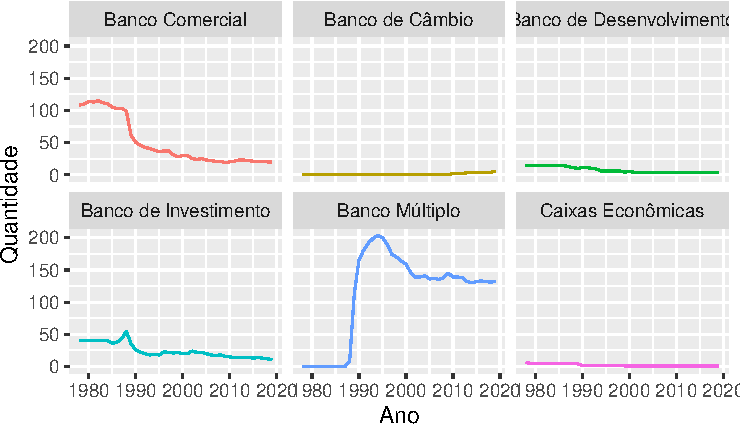
\includegraphics{12-exportedfigures/bank evolution-1} \end{center}
\label{fig:segmento}
\fonte{Desenvolvido a partir de dados do Banco Central}
\end{figure}

O índice de concentração Herfindahl--Hirschmanahl(HHI)\footnote{Desenvolvido pelos economistas Orris C. Herfindahl e Albert O. Hirschman, é utilizado amplamente para medidas de regulação da concorrência e leis antitrust}, refere-se a uma medida de concentração de mercado que mede a participação de uma determinada firma no mercado do qual participa. É obtida pela somatória quadrática da parcela de mercado a ser considerada, variando entre \(1/N\) e \(1\).
\[
HHI = \sum_{i=1}^{N}q_i^2
\]
A versão normalizada do HHI traz uma variação entre \(0\) e \(1\), perdendo em seu resultado a captação diante o número de firmas:
\[
HHIN = \frac{\frac{HHI - 1}{N}}{\frac{1-1}{N}}
\]
A versão decomposta do HHI avalia a assimetria da concentração de mercado inserindo um componente de variabilidade das participações das firmas, assim se verifica se as firmas possuem uma participação de mercado simétrica resultando em \(HHIN = 0\) e \(HHI= 1/N\).
\[
HHID = \frac{1}{N} + N\frac{\sum_{i=1}^{N}(\frac{q_i - 1}{N})^2}{N}
\]

A \autoref{fig:segmento} demonstra a evolução número de instituições bancárias
por segmento entre 1978 à 2019, podendo ser visualizada uma mudança na
composição da estrutura, com significativo aumento de instituições aderindo a
modalidades de múltiplas carteiras \footnote{As primeiras instituições com
carteira múltipla começaram a operar no ano de 1988} e redução de instituições que operam exclusivamente com carteira comercial e exclusivamente com carteira
de investimento.

\begin{table}
\caption{Composição por tipo de iniciativa no setor bancário brasileiro — Dezembro 2019}
\begingroup\fontsize{10}{12}\selectfont

\begin{tabu} to \linewidth {>{\raggedright\arraybackslash}p{6cm}>{\raggedright\arraybackslash}p{6cm}}
\toprule
Tipo & Participação\\
\midrule
\cellcolor{gray!6}{Privado} & \cellcolor{gray!6}{93\%}\\
Público & 7\%\\
\bottomrule
\end{tabu}
\endgroup{}
\label{tab:iniciativa}
\fonte{Desenvolvido pelo autor, com dados do Banco Central}
\end{table}

Alguns dos efeitos da abertura comercial-financeira e das modificações na
estrutura bancária provenientes das medidas governamentais foram o aumento da
participação de instituições estrangeiras no país e, um consistente processo de
fusões e aquisições, de ambas as origens de capital, que resultou em
considerável elevação do grau de concentração \cite{camargo:2009}.

\begin{figure}
\captionof{figure}{Evolução da quantidade de instituições no setor bancário brasileiro}

\begin{center}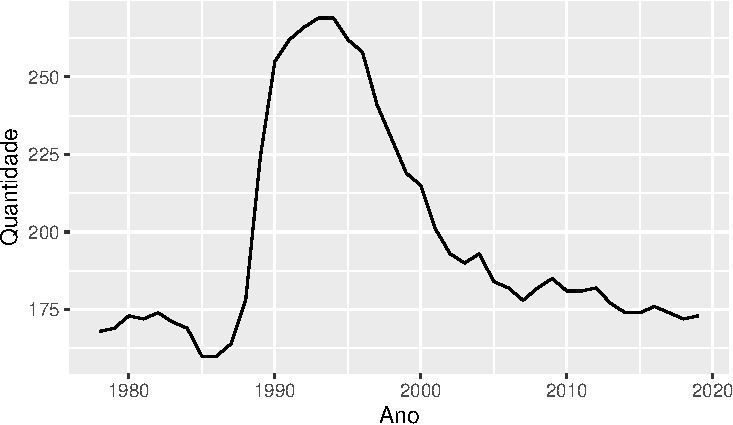
\includegraphics{12-exportedfigures/concetration-1} \end{center}
\label{fig:concentracao}
\fonte{Desenvolvido pelo autor, com dados do Banco Central}
\end{figure}

A observação sobre o aumento da concentração bancária no Brasil realizada por
\textcite{camargo:2009} pode ser visualizada na \autoref{fig:concentracao}.
Entre as metades das décadas de 1980 e 1990, com redução da concentração,
levando em consideração o número de instituições. Esse cenário passou se
inverter a partir de 1994, chegando em 2019 a um nível aproximado ao observado
no início da década de 1980.

De acordo com Strachman e Vasconcelos \emph{apud} \textcite{camargo:2009}, o aumento
da concentração bancária pode ser prejudicial ao crescimento econômico, uma vez
que, com maior participação de mercado, as instituições bancárias acabam por
obter a prerrogativa de determinar seus preços, comportamento este observado em
\textcite{klein:1971}.

Segundo \textcite{camargo:2009} e \textcite{dantas:2012} por outra perspectiva,
o ganho de escala, onde o cenário de aumento do tamanho das instituições, das
operações de crédito e redução de custos operacionais atua melhorando a
remuneração dos depósitos podendo atuar na redução dos juros finais pagos pelos
clientes.

Outra possível tendência para a concentração bancária seria a redução do risco
das operações, implicando em redução de custos, obtida por meio expansão
geográfica, setorial e de produtos financeiros. Porém os possíveis efeitos da
concentração dependem de uma série de condições, principalmente em torno da
eficiência e do nível de concorrência no mercado \cite{camargo:2009}.

\begin{table}
\caption{Setor bancário brasileiro por origem de capital — Dezembro de 2019}
\begingroup\fontsize{10}{12}\selectfont

\begin{tabu} to \linewidth {>{\raggedright}X>{\raggedleft}X>{\raggedright}X}
\toprule
Capital & Quantidade & Participação\\
\midrule
\cellcolor{gray!6}{Nacionais} & \cellcolor{gray!6}{66} & \cellcolor{gray!6}{43.1\%}\\
Controle Estrangeiro & 60 & 39.2\%\\
\cellcolor{gray!6}{Nacionais com Participação Estrangeira} & \cellcolor{gray!6}{12} & \cellcolor{gray!6}{7.8\%}\\
Públicos & 10 & 6.5\%\\
\cellcolor{gray!6}{Estrangeiros} & \cellcolor{gray!6}{5} & \cellcolor{gray!6}{3.3\%}\\
\bottomrule
\end{tabu}
\endgroup{}
\label{tab:origemcapital}
\fonte{Desenvolvida pelo autor, com dados do Banco Central}
\end{table}

\begin{figure}
\captionof{figure}{Evolução de origem de capital das instituições bancárias no Brasil}

\begin{center}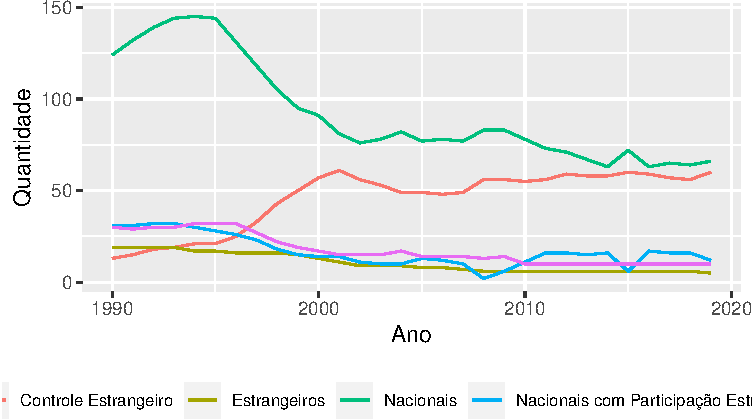
\includegraphics{12-exportedfigures/capital graphic-1} \end{center}
\label{fig:ev.capital}
\fonte{Desenvolvido pelo autor, com dados do Banco Central}
\end{figure}

O aumento da participação estrangeira no setor bancário brasileiro durante a
década de 1990, evidenciado por \textcite{camargo:2009} pode ser observado na
\autoref{fig:ev.capital}. Esse aumento ocorreu principalmente através do
controle acionário, com elevação acentuada na segunda metade da década de 1990
até o início da década de 2000. Ocorrendo redução em instituições
nacionais, estrangeiras e nacionais com participação estrangeira.

Durante este período, a inclinação para aplicação massiva em títulos públicos
se dava diante a manutenção de elevadas taxas de juros, tornando o crédito para
empreendimentos privados de elevado risco, e consequentemente elevando
substancialmente o \emph{spread} bancário e reduzindo a oferta de crédito
\cite{camargo:2009}.

A expectativa com a entrada de instituições estrangeiras era que houvesse
elevação da concorrência e, consequentemente, redução no \emph{spread} bancário,
aumento da concessão de crédito, melhoria da qualidade e diversificação dos
produtos financeiros, avanços em tecnologias, ou seja, uma elevação na
eficiência do setor \cite{camargo:2009}.

Porém, o que se observou foi a adoção de postura conservadora por partes dos
bancos estrangeiros, com estratégia de ativos inclinada para negociação de
títulos públicos, e passivos direcionados para a captação de recursos advindos
de grupos de rendas média e alta, com exceção dos bancos públicos que
concentraram em operações de crédito \cite{camargo:2009}.

\begin{figure}
\captionof{figure}{Evolução da relação Crédito/PIB no Brasil}

\begin{center}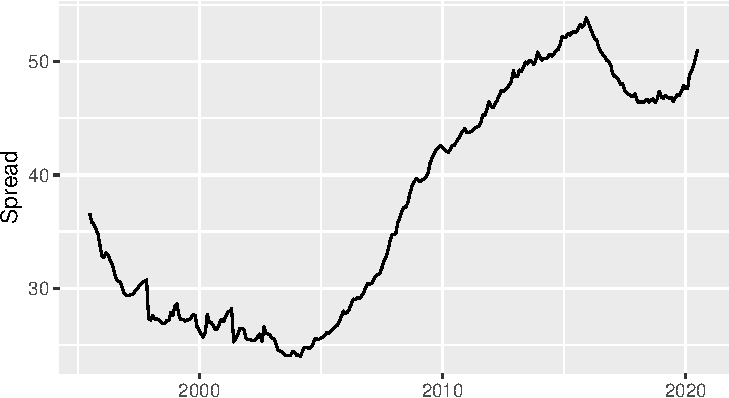
\includegraphics{12-exportedfigures/credit gdp-1} \end{center}
\label{fig:credgdp}
\fonte{Desenvolvido pelo autor, com dados o Banco Central}
\end{figure}

A \autoref{fig:credgdp} demonstra o comportamento da relação crédito/PIB no
Brasil, que entre a segunda metade da década de 1990 até a meados da primeira
metade da década de 2000 sofreu significativa queda, ficando abaixo dos 25\%.
Após esse período a oferta de crédito sofreu uma expansão exponencial atingindo
patamares acima de 50\% do PIB.

Durante o período citado, foi observado no setor bancário brasileiro os maiores
níveis de \emph{spread} praticados no mundo, associado a um quadro econômico
instabilidades e baixos crescimento e desenvolvimento. Esse cenário encontra
embasamento em estudos teóricos e empíricos que demonstram que um sistema
financeiro desenvolvido favorece o crescimento e desenvolvimento econômico
\cite{levine:1997, matos:2003}.

\begin{figure}
\captionof{figure}{Evolução anual do saldo carteira de crédito}

\begin{center}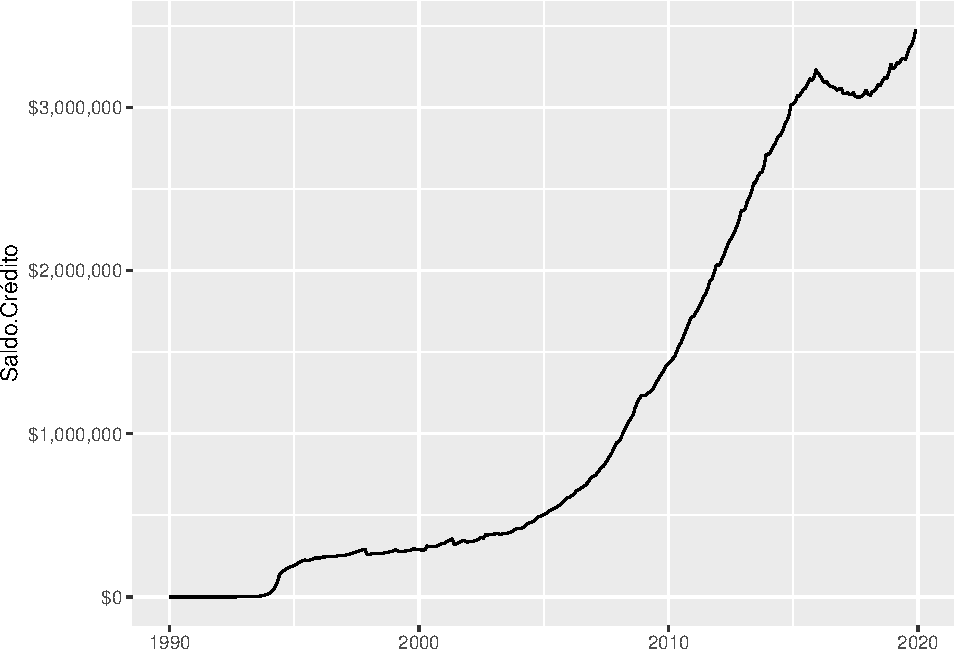
\includegraphics{12-exportedfigures/balance credit-1} \end{center}
\label{fig:saldocredito}
\fonte{Elaborado com dados do Banco Central}
\end{figure}

A \autoref{fig:saldocredito} demonstra a evolução do saldo da carteira de
crédito anual em termos correntes entre 1990 e 2020, podendo ser visualizada
uma expansão exponencial de crédito a partir do início da década de 2000, com
leve recuo na até metade da década de 2010 e retoma ultrapassando máxima
anterior.

Diante o levantamento, o setor bancário brasileiro durante o período avaliado
passou por diversas transformações em sua estrutura no que tange a concentração
de mercado, aumento da participação de capital estrangeiro por meio de controle
acionário, redução da participação pública.

Em relação aos indicadores foi verificado que, entre a década de 1980 até metade da década de 1990, no cenário hiperinflacionário, mesmo com redução da
concentração bancária, os indicadores de eficiência de intermediação
financeiras como o \emph{spread} bancário e a relação crédito/PIB estavam em níveis
considerados ineficientes e muito destoantes em comparação a outros países e
regiões.

A partir de 1995 se observou mudanças significativas no setor bancário, com
nova concentração, redução de instituições nacionais devido o controle
acionário por capital estrangeiro, e expressiva redução no \emph{spread} bancário e
a partir de 2004 uma mudança significativa na relação crédito/PIB.

O Sistema Financeiro como um todo, em sua organização entre agentes normatizadores, supervisores e operadores, além suas instâncias --- algumas já citadas ---, possui uma organização em torno da Base Monetária e dos Agregados Monetários, configurando a Oferta de Moeda de determinado País.

A Base Monetária (\(M_0\)) é configurada pelo total de cédulas e moedas em circulação no país e das Reservas Bancárias\footnote{São contas mantidas no Banco Central, obrigatória as instituições bancárias e consequentemente aos correntistas} --- em poder das instituições ou depositadas no Banco Central --- tido como emissão primária de moeda e configurando o passivo monetário, resultado líquido de todas as operações ativas e passivas do Banco Central. \cite{bcb:2019}.

\[
M_0 = PPE + RB
\]

Em 1995 foi introduzido um novo conceito de Base Monetária ampliada, que possui maior capacidade de explanar os preços da economia no Brasil, que o conceito restrito, uma vez que trazem maior percepção do fator substituição entre a moeda em seu conceito convencional e os demais ativos financeiros disponíveis, incluindo os passíveis como depósitos compulsórios e títulos públicos federais \cite{bcb:2019}.

Entre os Agregados Monetários estão o Meios de Pagamento na forma restrita (\(M_1\)), configurado por cédulas e moedas em poder dos agentes econômicos e seus depósitos à vista, que podem ser utilizados prontamente para pagamentos de bens e serviços. O conceito de Meios de Pagamentos Ampliado adiciona à moeda legal agregados que são considerados de elevada liquidez (\(M_2\)) e (\(M_3\)). \cite{bcb:2019}.

\[
M_1 = PMPP + DAV
\]

No conceito de Meio de Pagamento Ampliado o Agregado Monetário (\(M_2\)), contempla o Agregado Monetário \(M_1\) adicionado do resultante das emissões primárias por instituições depositárias no mercado interno, capazes de realizar a multiplicação de crédito, consistindo em depósitos especiais remunerados (\(DER\)), depósitos de poupança (\(DP\)) e títulos (\(TEID\)).

\[
M_2 = M_1 + DER + DP + TEID
\]

No conceito ampliado, o Agregado Monetário \((M_3)\) contempla o Agregado Monetário (\(M_2\)) adicionado das captações internas intermediadas pelos fundos de renda fixa e das carteiras de títulos públicos federais registrados no Sistema Especial de liquidação e e Custodia (Selic). Consiste em quotas de fundos de renda fixa (\(QFRF\)) e operações compromissadas registradas no Selic (operações compromissadas lastreadas em títulos públicos federais) (\(OCRS\)) \cite{bcb:2019}.

\[
M_3 = M_2 + QFRF + OCRS
\]

Existe ainda o conceito de poupança financeira composto pelo Agregado Monetário \(M_4\) contemplando o Agregado Monetário \(M_3\) mais a carteira livre de títulos públicos do setor não financeiro de elevada liquidez (\(CLSNF\)) \cite{bcb:2019} e o Agregado Monetário (\(M_5\)) que engloba o (\(M_5\)) mais a capacidade de aquisição de cartões de crédito (\(CACC\)) .

\[
M_4 = M_3 + CLSNF
\]
\[
M_5 = M_4 + CACC
\]

De acordo com a teoria quantitativa da moeda, o nível de preços (\(P\)) em uma economia guarda relação com a quantidade de moeda em circulação (\(M\)) e a velocidade (\(V\)) em que circula a moeda na economia --- frequência média em que uma unidade monetária é consumida em um período de tempo ---, diante o produto seu produto real (\(y\)), com a premissa que no curto prazo o produto e a velocidade a moeda são constantes \cite{vasconcellos:2011}.

\[
MV = Py => P = \frac{MV}{y} => V = \frac{Py}{M}\
\]

\begin{figure}
\captionof{figure}{Evolução da Base Monetária — no Brasil}

\begin{center}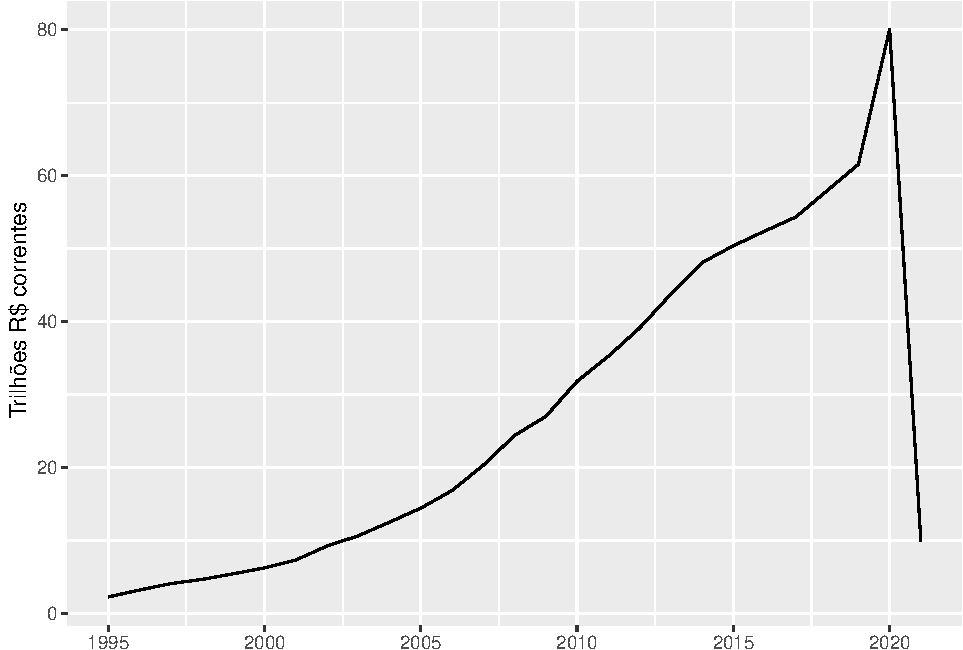
\includegraphics{12-exportedfigures/money-1} \end{center}
\label{fig:basemonet}
\fonte{Desenvolvido pelo autor, com dados o Banco Central}
\end{figure}

O gráfico \autoref{fig:basemonet} demonstra a evolução da Base Monetária entre os anos de 1995 e 2020 com elevação exponencial e constante durante este período, em termos constantes.

No que tange a abordagem microeconômica, as instituições bancárias como sociedade anônimas e instituições supervisionadas pelo Banco Central, são obrigadas a divulgar seus resultados em forma de demonstrações contábeis. A partir destas demostrações podem ser observados e extraídos dados e indicadores generalizados sobre a operação das instituições.

Os dados são divulgados seguindo uma padronização para o setor, onde podem ser observados as receitas, despesas, ativos, passivos, patrimônio líquido e a partir destes , calculados índices e indicadores, para cada período de registo, buscando refletir a situação econômica e financeira, podendo ser analisado de forma evolutiva e comparativa com outras instituições.

Entre os principais indicadores para avaliação de resultados das instituições bancárias, estão os índices de Liquidez Geral e Liquidez Corrente, Endividamento e Composição do Endividamento, retorno sobre o ativo, retorno sobre o patrimônio líquido, margem ebitda, margem líquida e grau de alavancagem financeira.

O índice de Liquidez Corrente (\(LC\)) mede a capacidade da instituição em honrar os compromissos com seus credores, definindo seu nível de solvência no curto prazo. É obtido pela razão entre o ativo circulante (\(AC\)) e o passivo circulante (\(PC\)), indicando o quanto do ativo circulante está disponível para cumprir com cada unidade monetária da dívida de curto prazo \cite{graham:2012} \cite{assaf:2020}.

\[
LC = \frac{AC}{PC}
\]
O índice de Liquidez Geral (\(LG\)) mede a capacidade da instituição honrar os compromissos com seus credores no longo prazo, definindo seu nível de solvência geral, é obtido pela razão entre a soma do ativo circulante (\(AC\)) e recursos realizáveis no longo prazo (\(RLP\)) e a soma do passivo circulante (\(PC\)) e exigível no longo prazo (\(ELP\)) \cite{assaf:2020}.

\[
LG_ = \frac{AC + RLP}{PC + ELP}
\]

O índice de endividamento (\(CT\)), mede a participação de capital de terceiros em relação aos financiamentos realizados com capital próprio. Quanto maior o indicador, maior a dependência da instituição de capital de terceiros para financiamento das suas operações, obtido pela razão entre o passivo (\(P\)) e o patrimônio líquido (\(PL\)) \cite{assaf:2020}.

\[
CT = [\frac{P}{PL}]
\]

A composição do endividamento (\(CE\)) indica o percentual da dívida da instituição em relação que vence no curto prazo. Quanto maior for esse indicador, mais crítica é a situação da instituição, necessitando de melhores resultados para cumprir os compromissos com credores no curto prazo, sendo obtido pela razão entre o passivo circulante (\(PC\)) e a soma do passivo ciculante e exigível a longo prazo (\(ELP\)) \cite{assaf:2020}.

\[
CE = \frac{PC}{PC + ELP}
\]

O Índice de Eficiência bancária (\(IE\)) é um indicador que avalia a relação entre despesas administrativas, despesas com pessoal e resultado operacional, medindo o quanto a instituição desembolsa para gerar uma unidade de receita. É obtido por meio da razão entre a soma das despesas administrativas (\(DA\)), despesas com pessoal (\(DP\)) líquidas da participação nos lucros (\(PLR\)) sobre a soma entre Margem Financeira (\(MF\)) e receita (\(R\)) \cite{timotio:2018}.

\[
IE = \frac{DA + DP - PLR}{MF + R} 
\]

Outro indicador utilizado para avaliação da situação financeira das instituições bancárias é o obtido da relação entre as receitas de prestação de serviços (\(RS\)) e as despesas administrativas (\(DA\)) \cite{dantas:2012}.

\[
RSDA = \frac{RPS_{}}{DA_{}}
\]

O retorno sobre o Ativo (\(ROA\)), mede a rentabilidade da instituição diante a totalidade dos seus ativos. O quanto para cada unidade monetária investida na instituição é convertida em lucro líquido, obtida da relação entre o lucro operacional (\(LO\)) e o ativo total (\(AT\)) \cite{assaf:2020}.

\[
ROA = \frac{LO}{AT}
\]

O Retorno sobre o Patrimônio Liquido (\(ROE\)) mensura a relação entre o lucro líquido (\(LL\)) em o Patrimônio Líquido (\(PL\)) da instituição, configurando o retorno dos investimentos para os sócios e acionista, para cada unidade monetária com recursos próprios aplicados na empresa \cite{assaf:2020}.

\[
ROE = \frac{LL}{PL}
\]

A margem EBITDA (\(MEB\)) é obtida da relação entre o EBITDA --- lucro antes dos juros, depreciação, amortização e impostos sobre a renda, configurando o lucro operacional da instituição --- e a Receita Líquida (\(RL\)), revelando a capacidade da instituição na geração de caixa \cite{assaf:2020}.

\[
MEB_it = \frac{EBITDA_it}{RL_it}
\]

A Margem Líquida (\(ML\)) é um indicador que demonstra a parte de cada unidade monetária das intermediações financeiras que foi convertida em Lucro Líquido, sendo obtida da relação entre o lucro líquido (\(LL\)) e O resultado líquido da intermediação financeira (\(RLIF\)) \cite{assaf:2020}.

\[
ML = \frac{LL}{RLIF}
\]

O grau de alavancagem financeira (\(GAF\)) consiste no indicador que captura o efeito da tomada de recursos de terceiros a um dado custo, alocados para ativos que possuam distintas taxas de retornos. Como se dá o aumento do lucro líquido através da estrutura de financiamento, definindo a parcela do retorno que seria melhor ou pior se estivessem financiando a operações totalmente com capital próprio \cite{assaf:2020}.

\[
GAF = \frac{RPL}{ROA}
\]

O risco de crédito das instituições bancárias pode ser obtido por meio da relação entre o saldo da Provisão para Créditos de Liquidação Duvidosa (\(PCLD\)) e do total da carteira de crédito (\(OPCR\)), obtidos através das contas 16900008 e 16000001 \cite{dantas:2012}

\[
RC_{} = \frac{PCLD_{}}{OPCR_{}}
\]

A participação de mercado (\(MS\)) de cada instituição pode ser mensurada a partir da relação entre suas operações de crédito \{\(OPCR\)\} no total das operações de crédito do mercado, sendo obtido através da conta 1600001 \cite{dantas:2012}.

\[
MS_{} = \frac{OPCR_{}}{\sum_{i}^{n}OPCR_{}} 
\]

Este capítulo levantou informações amplas sobre o setor bancário brasileiro, e
identificando e macroeconômicas e microeconômicas refrentes a economia como um todo, setor financeiro, ao setor bancário e as instituições em si. No próximo capítulo serão levantados conceitos, definições e estudos sobre a evolução, decomposição e determinantes do \emph{spread} bancário.

\textual
\pagestyle{simple}

\section{Spread Bancário}

Este capítulo irá tratar sobre os principais aspectos e características do
\emph{spread} bancário. Na primeira parte serão abordados conceitos e definições
gerais. Na segunda parte as características amplas do mercado Brasileiro. Na
terceira parte sobre os estudos empíricos realizados no Brasil. O foco é
identificar elementos que possam contribuir com o objeto deste estudo.

\subsection{Conceitos e Definições}

Por definição o \emph{spread} bancário é obtido através da subtração
entre a taxa de aplicação incidente nas operações de crédito, e a taxa de
captação que remunera as aplicações financeiras, se configurando como a
diferença entre a composição dos custos destas operações \cite{BCB:2000}.

\[
Spread = \text{Taxa de Aplicação} - \text{Taxa de Captação}
\]

O \emph{spread} bancário representa uma medida que sinaliza o desempenho dos bancos
\cite{levine:1997}. É considerado um indicador de eficiência da economia, no
sentido de favorecer o crédito e a atividade econômica. Em níveis elevados pode
desfavorecer o crédito destinado para produção e consumo produtivos e estar
associado com baixo desenvolvimento econômico \cite{WB:2005}.

Os estudos em torno do \emph{spread} bancário ocorrem em três óticas: evolução,
estrutura e determinantes (SOUZA (2014). Em Dick \emph{apud} \cite{leal:2006} é
destacada a importância de distinguir a abordagem em torno da estrutura e
determinante do \emph{spread} bancário, no sentido de complementariedade. O diagrama
na \autoref{fig:diagram} ilustra as óticas de estudo do \emph{spread} bancário.

\begin{figure}
\captionof{figure}{Diagrama de ilustração das vertentes de pesquisa do \emph{spread}}

\begin{center}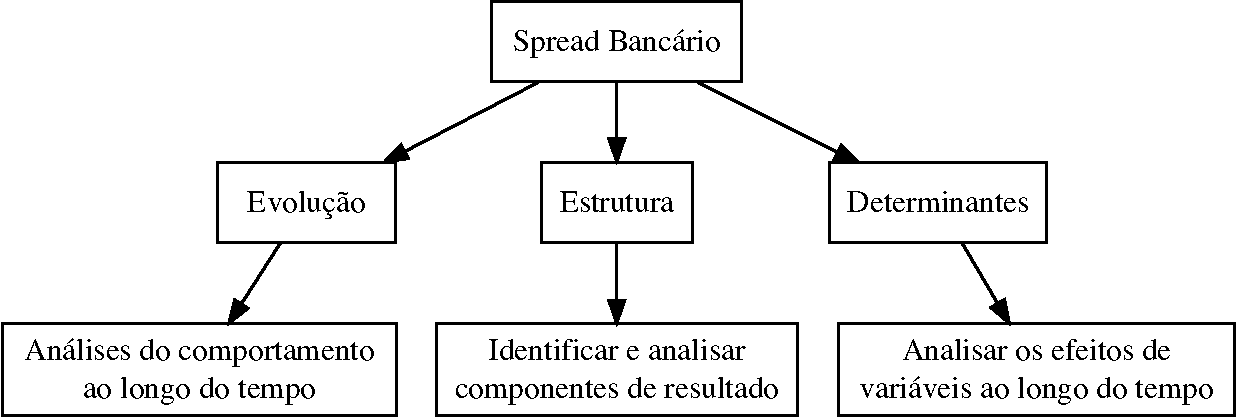
\includegraphics{12-exportedfigures/diagram.spread-1} \end{center}
\label{fig:diagram}
\fonte{Desenvolvido com base nas fontes citadas}
\end{figure}

A abordagem em torno da evolução visa analisar o comportamento ao longo do
tempo, através de análises quantitativas e qualitativas, enquanto a ótica da
estrutura busca identificar e analisar os componentes de resultado envolvendo
receitas, despesas e provisões. Na abordagem sobre os determinantes é
vislumbrado identificar as variáveis que explicam as variações do indicador ao
longo dos períodos \cite{leal:2006}.

Vem se tornando relevantes os estudos em torno da decomposição do \emph{spread}
bancário. Entre os componentes explícitos estão a inadimplência, despesas
administrativas, impostos diretos e indiretos e margem de lucro dos bancos
conforme ilustrado abaixo \cite{BCB:2000}.

\[
Sprd=f(Ind, DA, II, ML, CP)
\]

\begin{itemize}
\tightlist
\item
  Sprd = \emph{Spread}
\item
  Ind = Inadimplência
\item
  DA = Despesas Administrativas
\item
  II = Impostos Indiretos
\item
  ML = Margem de Lucro
\item
  CP = Custo de Captação
\end{itemize}

Esta configuração dos componentes, contemplando a margem de lucro, despesas e
riscos envolvidos nas operações de crédito vem desmistificar a comum abordagem
do \emph{spread} como o rendimento auferido pelos bancos \cite{costa;nakane:2004}
Souza (2007) \emph{apud} \cite{dantas:2012}. Desta forma se configurando como a
diferença entre o custos operacionais na ótica de precificação, que após
descontados das receitas, remontam o lucro do banco \cite{BCB:2016}.

Além da avaliação de seus componentes, o \emph{spread} pode ser analisado
conjuntamente por três características: enquanto a abrangência da amostra,
conteúdo e origem da informação \cite{leal:2006}.

A abrangência da amostra consiste nas especificidades das operações de crédito
das instituições e seu nível de agregação e granularidade
\cite{costa;nakane:2004}. Uma análise agregada dessa característica pode ser
dificultada pela existência de heterogeneidade do setor, ressaltando a
importância de realizar análises do \emph{spread} bancário em diferentes
características e óticas \cite{block:2000}.

A abordagem em torno do conteúdo está relacionada com os subcomponentes que
envolvem a receita e as despesas das intermediações financeiras, podendo
englobar, ou não, as tarifas e comissões sobre as taxas de captações e
aplicação \cite{block:2000}.

A origem da informação é analisada em dois cenários: \emph{ex-ante} e \emph{ex-post}
\cite{kunt:1999, levine:1997}. A perspectiva \emph{ex-ante} se refere as
expectativas das instituições bancárias em relação ao mercado de crédito e os
riscos envolvidos, obtido por método de precificação envolvendo as taxas de
captação e empréstimo \cite{durigan:2018, leal:2006, dantas:2012}.

O \emph{spread} \emph{ex-ante}, por se tratar de um indicador de planejamento, refletindo
as expectativas das instituições bancárias em relação ao mercado, finda
demonstrando-se mais volátil, não representando as taxas efetivas realizadas.
As informações \emph{ex-ante} são repassadas ao Banco Central que as divulgam
\cite{durigan:2018, leal:2006, dantas:2012}.

No \emph{spread ex-post} as margens são obtidas mediante a apuração dos resultados
contábeis, através dos demonstrativos, considerando as receitas e custos
efetivos, implicando nas taxas de intermediação e carteira realizadas pelas
instituições financeiras \cite{kunt:1999, durigan:2018}. Nesse sentido, em
termos médios, as taxas \emph{ex-post} se demonstram mais estáveis \cite{leal:2006, dantas:2012}.

O \emph{spread ex-post}, sendo resultante da diferença entre as taxas de empréstimos e de captação realizadas pelas instituições, é obtida por meio das contas 71100001, 16000001, 81100008 e 41000007 (das demonstrações contábeis padronizadas). O \emph{spread ex-post} se configura como o efetiva margem auferida pela instituição, diante seus resultados contabilizados \cite{dantas:2012}.

\[
SPR_it = [\frac{ROP_it}{\frac{OP_it + OP_it-1}{2}}] - [\frac{DOP_it}{\frac{DP_it + DP_it-1}{2}}]
\]
SPR = \emph{Spread ex-post}

ROP = Receitas das Operações de Crédito

OP = Operações de Crédito Média

DOC = Despesas das Operações de captação

DP = Depósitos médio

Reduções no \emph{spread} \emph{ex-post} não necessariamente significam aumento da
eficiência da intermediação financeira, pois podem estar associadas a uma
redução da inadimplência \cite{kunt:1999}. Como observado em
\textcite{klein:1971} e \textcite{ho-saunders:1981} o \emph{spread} bancário é
determinado de acordo com as características e os riscos envolvidos nas
intermediações financeiras inerentes em cada estrutura de mercado.

\subsection{Spread Bancário no Brasil}

No Brasil, a taxa de aplicação para crédito de recursos livres é pactuado entre
instituição e tomador. Somente as operações de crédito envolvendo recursos
direcionados são sujeitas à limites, não podendo exceder 12\%a.a. mais a taxa
referencial de juros \cite{BCB:2016}.

No mercado bancário Brasileiro, o modelo consolidado de mensuração do \emph{spread},
conforme \autoref{tab:spread.tb}, leva em consideração o saldo médio de capital
emprestado, e a diferença entre as receitas de aplicação e despesas de
captação, ocorrendo a classificação em \emph{spread} bruto, direto e líquido
\cite{fipecafi:2005}

\begin{table}[b]
 \centering
   \captionof{table}{Esquema de obtenção do \emph{spread} mais adotado no mercado} 
    \label{tab:spread.tb}
     \begin{tabular}{l|r|r|r}
      \hline
                                           &   PJ   &   PF    & Total \\
       \hline
       Saldo Médio do Capital Emprestado   & 100.00 & 100.00  & 100.00 \\
       A — Receita de Aplicação Financeira & 9.4    & 16.5    & 12,7   \\
       B — Despesas de Captação            & (4.8)  & (4.9)   & (4.8)  \\   
       Spread Bruto                        & 4.6    & 11.6    & 7.9    \\
       Spread Direto                       & 3.2    & 7.6     & 5.3    \\
       Spread Líquido                      & 0.5    & 1.6     & 1.0    \\
       \hline
       \end{tabular}
\fonte{in \cite{fipecafi:2005}}
\end{table}

O Banco Central, em 1999, iniciou uma série de estudos e medidas com objetivo
de reduzir a taxa de juros e o \emph{spread} realizados no setor bancário
Brasileiro, atuando na identificação e ajustes em variáveis econômicas
influentes. Entre as primeiras medidas estavam a redução da taxa de compulsório
para depósitos à vista e até a extinção para depósitos à prazo, redução do IOF
e a redução da Selic \cite{BCB:2000}.

\begin{figure}
\captionof{figure}{Evolução do \emph{spread} bancário Brasileiro até 2011}

\begin{center}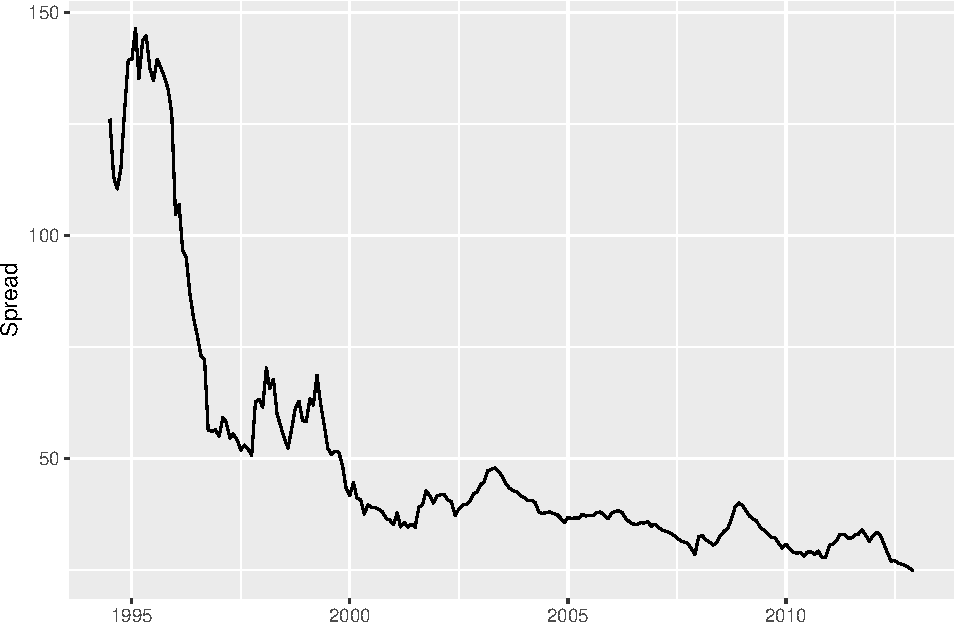
\includegraphics{12-exportedfigures/average spread-1} \end{center}
\label{fig:spread2012}
\fonte{Desenvolvido a partir de dados do Banco Central}
\end{figure}

A \autoref{fig:spread2012} mostra a evolução do \emph{spread} bancário Brasileiro
médio entre os anos de 1994 e 2012, chegando a atingir 146.44\%, com
significativa queda ao longo desse período, atingindo 24.69\% no final
do período. Esta série foi descontinuada em 2012, passando a ser utilizada nova
metodologia de cálculo.

O Banco Central, até 2007 utilizava metodologia para avaliação do spread
bancário contemplando somente os recursos livres, o que não vinha a
proporcionar uma avaliação mais aprofundada. Em 2008 houve uma modificação na
metodologia de decomposição do \emph{spread}, alterando o cálculo do custo médio de
captação e detalhando classificações do crédito \cite{dantas:2012}

Para o custo médio de captação passou a se utilizar a taxa média ponderada
entre as taxas dos depósitos à prazo (CDB), em caderneta de poupança e à vista,
a participação dos custos efetivos dos recolhimentos compulsórios em detrimento
do custo de oportunidade \cite{dantas:2012}

O BACEN mantém atualmente duas séries para o indicador: spread médio das
operações de crédito (MOC) e Spread do Indicador de Custo de Crédito (ICC). As
séries são disponibilizadas em termos totais e nas subdivisões de tipo de
recursos, tipo de crédito e tomador.

Estas séries estatísticas representam estimativas baseadas nas informações
repassadas pelas instituições bancárias das taxas de juros das operações de
crédito e indicadores do mercado financeiro do custo médio do dinheiro para o
custo médio de captação \cite{BCB:2016}.

A série do Spread médio das operações de crédito é calculada a partir da
diferença entre a taxa média de juros de novas operações de crédito no SFN e o
custo de captação referencial médio de operações de crédito livre, direcionado
e não rotativo podendo ser observados por tomador.

\begin{figure}
\captionof{figure}{Evolução do Spread médio das operações de crédito}

\begin{center}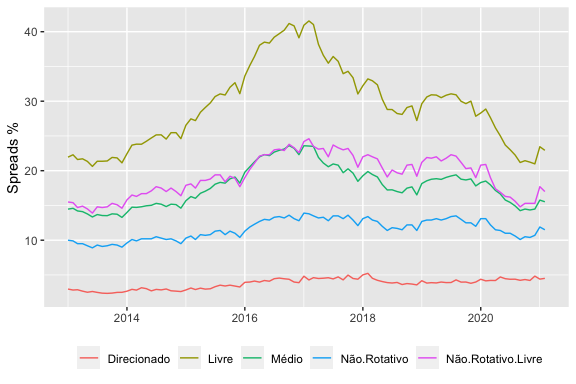
\includegraphics{12-exportedfigures/spread 2019 moc-1} \end{center}
\label{fig:spreadmoc}
\fonte{Desenvolvido a partir de dados do Banco Central do Brasil — Departamento de Estatísticas}
\end{figure}

A \autoref{fig:spreadmoc} mostra a visualização da evolução mensal do spread
médio das novas operações de crédito contratadas entre janeiro de 2013 e julho
de 2020. No período entre 2014 e 2017 se visualiza uma elevação de 10 p.p no
spread total, recuando 8 p.p a patamar próximo ao início do período. É possível
notar a grande disparidade entre os spread de recursos livres e direcionados.

A série do Spread do ICC, considera a diferença entre o Índice de Custo de
Crédito --- equivalente ao custo médio de juros das operações ativas da carteira
do SFN --- e o custo de captação médio ponderado, levando em consideração
operações de crédito livre, direcionado e não rotativo, dividido em pessoa
física e jurídica.

\begin{figure}
\captionof{figure}{Evolução do Spread do Índice do Custo de Crédito}

\begin{center}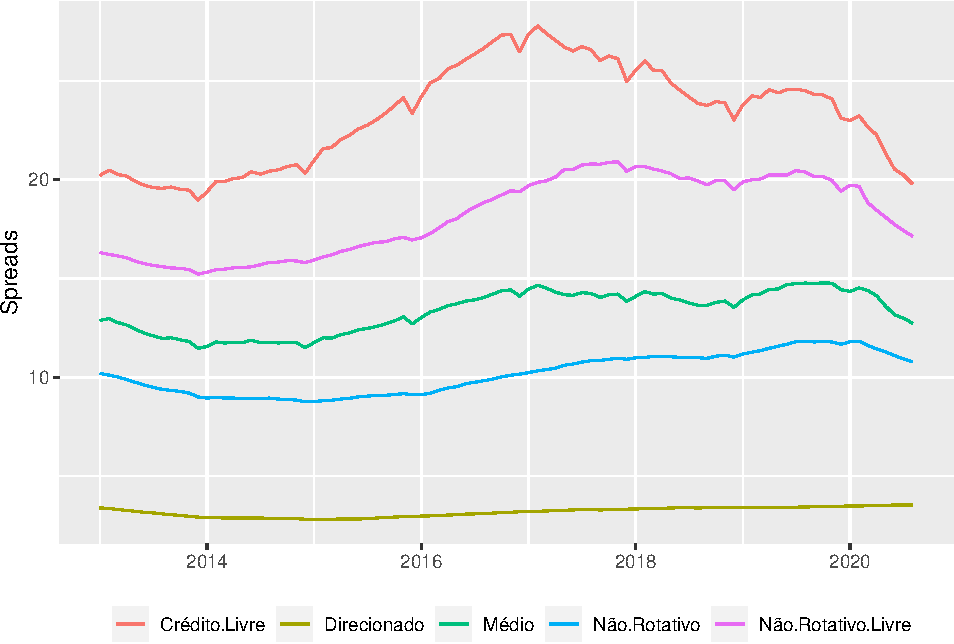
\includegraphics{12-exportedfigures/spread 2019 icc-1} \end{center}
\label{fig:spreadicc}
\fonte{Desenvolvido a partir de dados do Banco Central do Brasil - Departamento de Estatísticas}
\end{figure}

Na \autoref{fig:spreadicc} pode ser visualizada a evolução do spread do ICC,
entre janeiro de 2013 e julho de 2020 com expressiva elevação entre 2014 e
2017, passando a decair até retormar a patamares similares ao início do
período. Também pode ser notado a significativa diferença entre os \emph{spreads} de
recursos livres e direcionados.

O Indicador Custo de Crédito (ICC) consiste no custo médio de todas as
operações de crédito abertas --- independentes do período em que foram
contratadas --- que compõem a carteira de empréstimos, financiamentos e
arrendamento mercantil das instituições do Sistema Financeiro Nacional (SFN) \cite{BCB:2000}.

\begin{figure}
\captionof{figure}{Evolução do Indicador de Custo de Crédito (ICC)}

\begin{center}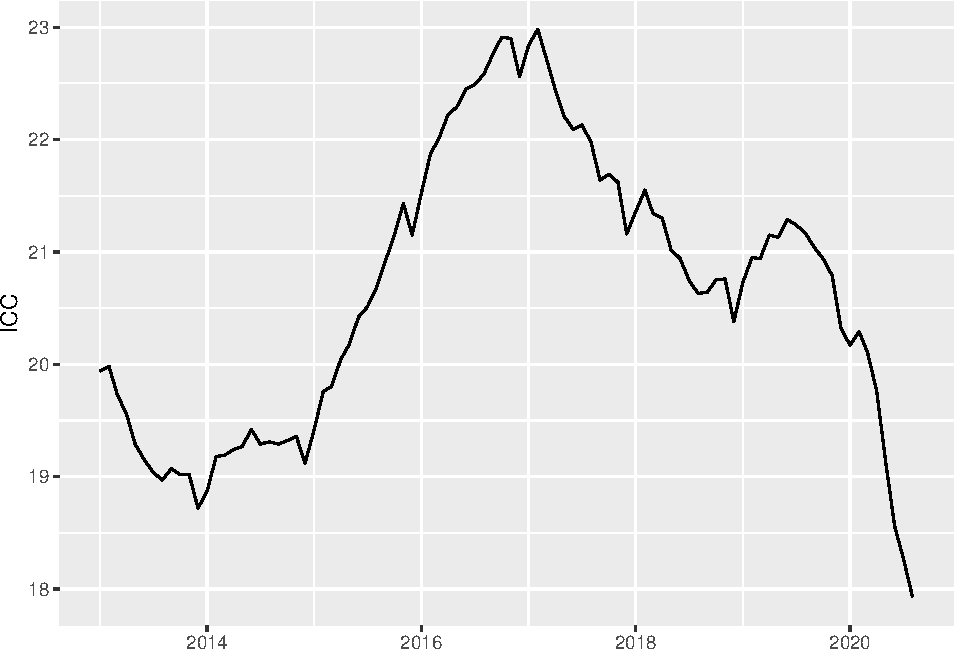
\includegraphics{12-exportedfigures/ICC-1} \end{center}
\label{fig:evicc}
\fonte{Desenvolvido a partir de dados do Banco Central do Brasil — Departamento de Estatísticas}
\end{figure}

A \autoref{fig:evicc} traz a visualização da evolução do Índice de Custo de
Crédito entre janeiro de 2013 e agosto de 2020, com máxima de 22.98\% em
2017, com queda significativa a partir de 2020, chegando a atingir 16.91\%
em agosto de 2020.

\subsection{Estudos anteriores}

Na literatura acadêmica não existe uma teoria formalizada acerca do \emph{spread}
bancário \cite{timotio:2018}. Sendo verificados estudos empíricos que visam
classificar, analisar e identificar variáveis micro e macroeconômicas
influentes nesse indicador em diversas perspectivas.

A grande maioria dos estudos realizados no Brasil utilizam as medidas de
\emph{spread} bancário divulgadas pelo Banco Central, que remetem a uma perspectiva
\emph{ex-ante}, registrando as taxas planejadas na fase de concessão de crédito. E
para as variáveis explicativa a grande maioria utiliza indicadores
macroeconômicos \cite{dantas:2012}

No ano de 1994, \textcite{aronovich:1994} realizou estudo econométrico para
verificar a influência da inflação e nível de atividade econômica no \emph{spread}
bancário ex-ante, encontrando relação direta do \emph{spread} com a inflação e
indireta com o nível de atividade econômica.

Em estudo dos determinantes macroeconômicos do \emph{spread} bancário ex-ante,
\textcite{oreiro-2006} utilizou regressão múltipla para identificar as
variáveis influentes (modelo abaixo). O estudo chegou ao resultado que alta
volatilidade e as taxas da Selic são um dos principais determinantes desse
indicador no setor bancário Brasileiro, identificando também a significância do
nível de atividade industrial.

\[
ln spread = \beta_0 trend + \beta_1 ln selic + \beta_2 ln adm + \beta_3 ln risk + \beta_4 ln imp + \beta_5 ln comp
\]

\begin{itemize}
\tightlist
\item
  \(\beta_i\) (i= 0,\ldots{}, 5) = parâmetros estimados;
\item
  trend = tendência determinista que controla outras variáveis;
\item
  selic = taxa Selic;
\item
  adm = despesa administrativas;
\item
  risk = proxy para o risco de crédito (spread do C-Bond sobre o rendimento dos títulos do Tesouro Americano de mesma maturidade;
\item
  imp são impostos indiretos;
\item
  comp = compulsório incidente sobre os depósitos à vista.
\end{itemize}

Em análise dos determinantes do \emph{spread} bancário ex-post,
\textcite{dantas:2012} utilizou variáveis explanatórias microeconômicas de cada
instituição, por meio de dados em painel dinâmico, entre janeiro de 2000 e
outubro de 2009, encontrando níveis significativos e diretos com o risco de
crédito, grau de concentração e nível de atividade econômica, e indireta com a
participação da instituição no mercado, não encontrando níveis significativos
com origem de capital e tipo de organismo.

Outra observação em \textcite{dantas:2012} foi a forte relação do \emph{spread}
\emph{ex-post} no momento atual com o momento anterior imediato, e que as
instituições tendem a cobrar maiores taxas, quando maior o nível de
concentração do mercado, não encontrando significância da Selic na determinação
deste indicador.

Em \textcite{almeida:2013} foi desenvolvido modelo de dados macroeconômicos e
microeconômicos em painel, de 64 instituições bancárias para avaliação de
determinantes do \emph{spread} \emph{ex-post} no Brasil entre o primeiro trimestre de
2001 e o segundo trimestre de 2012, encontrando como relevantes
as despesas administrativas, receita de serviços, índice de cobertura, PIB e o
grau de concentração.

Em \textcite{durigan:2018} foi realizada análise dos fatores macroeconômicos e
indicadores industriais que influenciam o \emph{spread} bancário ex-ante, através de
análise de regressão linear multivariada utilizando 18 variáveis em quatro
modelos. Chegando a conclusão que o aumento da atividade industrial, a redução
do desemprego e o consumo atuam na diminuição do \emph{spread} bancário.

Os modelos desenvolvidos por \textcite{durigan:2018} demonstraram que há uma
relação significativa e direta entre \emph{spread} e: inadimplência, IPIs (bens de
capital, intermediários, semiduráveis, não duráveis e consumo duráveis), Selic,
PIB, desemprego e o EMBI+ (medida de taxa de risco-país). As relações indiretas
com o \emph{spread} foram encontradas: no IPI de bens de consumo e geral, IPCA,
saldo da carteira de crédito e índice de vendas no varejo.

O estudo de \textcite{timotio:2018} teve foco em abordagem microeconômica, ao
buscar identificar a influência das variações de indicadores
financeiros-contábeis no \emph{spread} em 26 instituições bancárias,
através de regressão em dados em painel. Encontrando relações significativas
diretas com a alavancagem financeira, retorno sobre o patrimônio líquido,
EBITDA, Ativo Total e eficiência.

No modelo de \textcite{timotio:2018} foi encontrada relação significativa e
indireta do \emph{spread} com a participação de capital de terceiros e, não
identificada relação significativa com a composição do endividamento, retorno
sobre ativos e a liquidez corrente.

De acordo com \textcite{durigan:2018, dantas:2012}, existem poucos estudos
inclinados para os determinantes do \emph{spread} \emph{ex-post} no Brasil, onde
identificaram o estudos de Guimarães (2002). Foram identificados ainda os
estudos acerca do \emph{spread} ex-pots de Fipecafi (2004) \emph{apud}
\textcite{dantas:2012} e Matias (2006) \emph{apud} \textcite{leal:2006}

Em \textcite{fipecafi:2005} foi realizado estudo de apuração de resultados,
ex-post, baseado em demonstrações contábeis entre o 1º semestre de 2005 de
instituições que representavam 75,8\% do ativo total e 76\% do total de crédito.
Chegando a um resultado médio de \emph{spread} bruto de 7,6\% para pessoa física e
3,2\% para pessoa jurídica, e \emph{spread} líquido de 1,6\% para pessoa física e 0,5\%
para pessoa jurídica.

A \autoref{tab:exantea} e a \autoref{tab:exanteb} trazem o resumo dos
principais estudos empíricos sobre \emph{spread} bancário ex-ante no Brasil, com
resultados obtidos através de modelagem econométrica com utilização de
regressão, tomando variáveis micro e macroeconômicas como explanatórias e
demonstrando a relação com o spread ex-ante.

\begin{table}
\caption{Resumo de estudos sobre o \emph{spread ex-ante} no Brasil — Parte 1}
\begin{table}[H]
\centering\begingroup\fontsize{10}{12}\selectfont

\begin{tabular}[t]{>{\raggedright\arraybackslash}p{4cm}>{\raggedright\arraybackslash}p{2cm}>{\raggedright\arraybackslash}p{2cm}>{\raggedright\arraybackslash}p{2cm}>{\raggedright\arraybackslash}p{2cm}}
\toprule
Variável & KOYAMA e NAKANE (2001a e 2001b) & AFANASIEFF, LHAGER e NAKANE (2001) & AFANASIEFF, LHAGER e NAKANE (2002) & BIGNOTTO e RODRIGUES (2006)\\
\midrule
\textbf{\cellcolor{gray!6}{Custos Administrativos}} & \cellcolor{gray!6}{+} & \cellcolor{gray!6}{+} & \cellcolor{gray!6}{+} & \cellcolor{gray!6}{+}\\
\textbf{IGP} & + & + & - & \\
\textbf{\cellcolor{gray!6}{Impostos Indiretos}} & \cellcolor{gray!6}{+} & \cellcolor{gray!6}{+} & \cellcolor{gray!6}{+} & \cellcolor{gray!6}{}\\
\textbf{Requerimento de Reserva} & + &  &  & \\
\textbf{\cellcolor{gray!6}{Selic}} & \cellcolor{gray!6}{+} & \cellcolor{gray!6}{+} & \cellcolor{gray!6}{+} & \cellcolor{gray!6}{+}\\
\addlinespace
\textbf{Spread Over Treasury} & + &  & + & \\
\textbf{\cellcolor{gray!6}{Produto Industrial}} & \cellcolor{gray!6}{-} & \cellcolor{gray!6}{} & \cellcolor{gray!6}{} & \cellcolor{gray!6}{}\\
\textbf{Ativo Total} &  &  &  & +\\
\textbf{\cellcolor{gray!6}{Bancos Estrangeiros}} & \cellcolor{gray!6}{} & \cellcolor{gray!6}{} & \cellcolor{gray!6}{-} & \cellcolor{gray!6}{}\\
\textbf{Captação sem juros} &  & + & + & \\
\addlinespace
\textbf{\cellcolor{gray!6}{Compulsório}} & \cellcolor{gray!6}{} & \cellcolor{gray!6}{} & \cellcolor{gray!6}{} & \cellcolor{gray!6}{+}\\
\textbf{Crescimento PIB Industrial} &  & - & + & \\
\textbf{\cellcolor{gray!6}{IPCA}} & \cellcolor{gray!6}{} & \cellcolor{gray!6}{} & \cellcolor{gray!6}{} & \cellcolor{gray!6}{-}\\
\textbf{Liquidez} &  &  &  & +\\
\textbf{\cellcolor{gray!6}{Market Share}} & \cellcolor{gray!6}{} & \cellcolor{gray!6}{} & \cellcolor{gray!6}{} & \cellcolor{gray!6}{-}\\
\addlinespace
\textbf{Receita Serviços} &  & + & + & +\\
\textbf{\cellcolor{gray!6}{Risco Crédito}} & \cellcolor{gray!6}{} & \cellcolor{gray!6}{} & \cellcolor{gray!6}{} & \cellcolor{gray!6}{+}\\
\textbf{Risco Juros} &  &  &  & +\\
\textbf{\cellcolor{gray!6}{Volatilidade da Selic}} & \cellcolor{gray!6}{} & \cellcolor{gray!6}{-} & \cellcolor{gray!6}{} & \cellcolor{gray!6}{}\\
\bottomrule
\end{tabular}
\endgroup{}
\end{table}
\label{tab:exantea}
\fonte{Desenvolvido a partir das fontes citadas}
\end{table}

Entre os estudos da \autoref{tab:exantea} e \autoref{tab:exanteb} que avaliaram
a Selic e as despesas administrativas, há um consenso que estas variáveis
possuem uma relação de determinação direta com o \emph{spread ex-ante}. Em três
estudos que avaliaram impostos indiretos e receita de serviços foi encontrada
relação direta com o \emph{spread ex-ante}.

\begin{table}
\caption{Resumo de estudos sobre o \emph{spread ex-ante} no Brasil — Parte 2}
\begin{table}[H]
\centering\begingroup\fontsize{10}{12}\selectfont

\begin{tabular}[t]{>{\raggedright\arraybackslash}p{4cm}>{\raggedright\arraybackslash}p{3cm}>{\raggedright\arraybackslash}p{3cm}>{\raggedright\arraybackslash}p{3cm}}
\toprule
Variável & OREIRO et al. (2006) & DURIGAN (2018) & ARONOVICH (1994)\\
\midrule
\textbf{\cellcolor{gray!6}{Selic}} & \cellcolor{gray!6}{+} & \cellcolor{gray!6}{+} & \cellcolor{gray!6}{}\\
\textbf{Produto Industrial} & + &  & \\
\textbf{\cellcolor{gray!6}{Atividade Econômica}} & \cellcolor{gray!6}{} & \cellcolor{gray!6}{} & \cellcolor{gray!6}{-}\\
\textbf{Desemprego} &  & + & \\
\textbf{\cellcolor{gray!6}{EMBI}} & \cellcolor{gray!6}{} & \cellcolor{gray!6}{+} & \cellcolor{gray!6}{}\\
\addlinespace
\textbf{Inadimplência} &  & + & \\
\textbf{\cellcolor{gray!6}{Índice Volume Vendas Varejo}} & \cellcolor{gray!6}{} & \cellcolor{gray!6}{-} & \cellcolor{gray!6}{}\\
\textbf{IPCA} &  & - & +\\
\textbf{\cellcolor{gray!6}{IPI bcd}} & \cellcolor{gray!6}{} & \cellcolor{gray!6}{+} & \cellcolor{gray!6}{}\\
\textbf{IPI Bens de Capital} &  & + & \\
\addlinespace
\textbf{\cellcolor{gray!6}{IPI Bens de Consumo}} & \cellcolor{gray!6}{} & \cellcolor{gray!6}{-} & \cellcolor{gray!6}{}\\
\textbf{IPI Bens i} &  & + & \\
\textbf{\cellcolor{gray!6}{IPI bsd}} & \cellcolor{gray!6}{} & \cellcolor{gray!6}{+} & \cellcolor{gray!6}{}\\
\textbf{IPI Geral} &  & - & \\
\textbf{\cellcolor{gray!6}{IPIad}} & \cellcolor{gray!6}{} & \cellcolor{gray!6}{+} & \cellcolor{gray!6}{}\\
\addlinespace
\textbf{PIB} &  & + & \\
\textbf{\cellcolor{gray!6}{Saldo Carteira Crédito RL}} & \cellcolor{gray!6}{} & \cellcolor{gray!6}{-} & \cellcolor{gray!6}{}\\
\textbf{Volatilidade da Selic} & + &  & \\
\bottomrule
\end{tabular}
\endgroup{}
\end{table}
\label{tab:exanteb}
\fonte{Desenvolvido a partir das fontes citadas}
\end{table}

Ainda analisando a \autoref{tab:exantea} e a \autoref{tab:exanteb}, dois
estudos chegaram a resultados diferentes para os efeitos da volatilidade da
Selic no \emph{spread ex-ante}. Os efeitos do IPCA foram testados em três estudos,
os dois mais recentes encontraram uma relação indireta com a variável
dependente. Em três estudos que examinaram o IGP, dois encontram relação
direta, sendo que um deles foi repetido em período anterior e encontrou relação
indireta.

\begin{table}
\caption{Resumo de estudos sobre o \emph{spread ex-post} no Brasil}
\begin{table}[H]
\centering\begingroup\fontsize{10}{12}\selectfont

\begin{tabular}[t]{>{\raggedright\arraybackslash}p{4cm}>{\raggedright\arraybackslash}p{3cm}>{\raggedright\arraybackslash}p{3cm}>{\raggedright\arraybackslash}p{3cm}}
\toprule
Variável & GUIMARÃES (2002) & DANTAS (2012) & ALMEIDA (2013)\\
\midrule
\textbf{\cellcolor{gray!6}{Custos Administrativos}} & \cellcolor{gray!6}{} & \cellcolor{gray!6}{} & \cellcolor{gray!6}{+}\\
\textbf{Impostos Indiretos} &  &  & Não significativo\\
\textbf{\cellcolor{gray!6}{Requerimento de Reserva}} & \cellcolor{gray!6}{} & \cellcolor{gray!6}{} & \cellcolor{gray!6}{+}\\
\textbf{Atividade Econômica} &  & + & \\
\textbf{\cellcolor{gray!6}{Bancos Estrangeiros}} & \cellcolor{gray!6}{+} & \cellcolor{gray!6}{} & \cellcolor{gray!6}{}\\
\addlinespace
\textbf{Caixa.Depósitos} & + &  & \\
\textbf{\cellcolor{gray!6}{Grau Concentração}} & \cellcolor{gray!6}{} & \cellcolor{gray!6}{+} & \cellcolor{gray!6}{+}\\
\textbf{Liquidez} &  &  & Não significativo\\
\textbf{\cellcolor{gray!6}{Market Share}} & \cellcolor{gray!6}{} & \cellcolor{gray!6}{-} & \cellcolor{gray!6}{+}\\
\textbf{PIB} &  &  & +\\
\addlinespace
\textbf{\cellcolor{gray!6}{Receita Serviços}} & \cellcolor{gray!6}{} & \cellcolor{gray!6}{} & \cellcolor{gray!6}{-}\\
\textbf{Risco Crédito} &  & + & Não significativo\\
\bottomrule
\end{tabular}
\endgroup{}
\end{table}
\label{tab:expost}
\fonte{Desenvolvido a partir das fontes citadas}
\end{table}

A \autoref{tab:expost} traz o resumo dos estudos empíricos dos determinantes do
\emph{spread ex-post} no Brasil, por meio de modelos econométricos utilizando
regressão. Destaca-se que, entre os estudos, dois encontraram significância de
influência direta com o grau de concentração e o \emph{spread} ex-post. E dois dos
estudos chegaram a resultados opostos para os de posição de market share e a
variável dependente.

Este capítulo verificou os principais conceitos, características e estudos
acerca do \emph{spread} bancário no Brasil, identificando as óticas de análise por
evolução, composição e determinantes através da abrangência da amostra,
conteúdo e origem da informação. E que as maiores limitações estão na
dificuldade de desagregação de informações para uma análise mais aprofundada.

No próximo capítulo, será descrita a metodologia de trabalho com a formulação
das hipóteses baseado nas informações e levantamentos dos capítulos anteriores,
nos estudos pesquisados e na teoria econômica, através da coleta, tratamento e
análise de dados.

\textual
\pagestyle{simple}

\chapter{Procedimentos Metodológicos}

Neste capítulo serão descritos os principais procedimentos metodológicos,
técnicas e ferramentas que serão utilizados neste trabalho, visando organizar as etapas da pesquisa e permitir um maior nível de reproducibilidade, revisão e
refutabilidade da mesma.

Este trabalho está sendo desenvolvido e editado em ambiente R Markdown com utilização de linguagem Latex para padronização de textos, figuras e tabelas, e as linguagens R e Python para coleta, limpeza, tratamento, análise, visualização e modelagem e estimação econométrica dos conjuntos de dados.

Serão selecionadas as instituições bancárias na categoria de Banco Comercial, Banco e Investimento, Banco de Desenvolvimento e Caixa Econômicas que realizaram operações de crédito. Para fins de análise de dados, este trabalho atuará no intervalo de tempo entre o primeiro trimestre de 1999 e o terceiro trimestre e 2020.

Para efeitos de identificação de variáveis macroeconômicas que atuam como componentes implícitos e explícitos do \emph{spread} serão avaliadas a taxa Selic, Taxa de Compulsório, Base Monetária, Oferta de Crédito, Oferta de Moeda. Estes dados serão obtidos de forma secundária nos bancos de dados abertos do Banco Central, IPEA, IBGE e Receita Federal do Brasil.

Os dados de resultados, operação, indicadores e estrutura de capital das instituições bancárias serão obtidos de forma secundária nos banco de dados abertos do Banco Central e da Comissão de Valores Monetários, consistindo em demonstrações contábeis trimestrais padronizadas informadas a estas instituições supervisoras.

Para construção dos modelos econométricos a serem estimados se partirá de alguns pressupostos teóricos norteadores obtidos através da pesquisa bibliográfica e concepções desenvolvidas antes e durante a pesquisa, com intuíto embasar a seleção das variáveis a serem testadas e incluídas no modelo final.

Será assumido que o \emph{spread} bancário é definido diante um conjunto de fatores endógenos, definidos por questões microeconômicas envolvendo as operações de cada instituição e dos mercados financeiro e bancário, e fatores exógenos provenientes de questões macroeconômicas, afetando diretamente ou indiretamente as operações.

O \emph{spread} (\(SPR\)) será abordado dentro de uma concepção de precificação, diante um conjunto de variáveis explícitas como despesa de captação (\(D\)), capital emprestado (\(E\)) --- insumo das operações de crédito ---, impostos variáveis (\(II\)), despesas administrativas (\(DA\)), lucro líquido (\(ML\)) e inadimplência (\(IND\)).

\[
Spr = f(E,D,II,DA,ML,IND)
\]

Na visão microeconômica, assume-se que o \emph{spread} bancário não se configura na margem de lucro dos bancos, não cabendo abordagem de \emph{spread} bruto, direto e líquido. E que o \emph{spread} bancário se relaciona com os resultados das instituições, colaborando com a solidez do setor, não cabendo a inclusão no modelo de variáveis que rementam a resultados e calculadas a partir destas.

Na abordagem macroeconômica, o \emph{spread} bancário é tido como um indicador fundamental e determinante para o nível de desenvolvimento econômico de determinado país ou região a medida que se relaciona com a determinação de nível e crédito produtivo capaz de gerar renda, influenciado por variáveis macroeconômicas relacionadas a regulação e políticas monetárias e e fiscais.

Nesse sentido aqui é estabelecida a compreensão que o nível de atividade econômica, industrial, produtividade, desemprego e produto interno bruto de mercados, países e regiões guardam relação com o \emph{spread} bancário, e não o contrário, mesmo que aja a compreensão da abordagem em torno das expectativas dos agentes, será mantida a abordagem econômica, não considerando essas variáveis como determinantes do \emph{spread ex-post}.
\[
SprEp = f(SEL,COMP,IPCA,BM,MP,VM)
\]

O primeiro modelo a ser desenvolvido buscará testar e selecionar variáveis macroeconômicas e microeconômicas que exerçam significativa influência, de forma implícita e explícita no \emph{spread} bancário \emph{ex-post}. Partindo da definição geral tautológica de \emph{Spread} (\(Spr\)), resultado da diferença entre a taxa de aplicação (\(I_{apl}\)) e a taxa de captação (\(i_{cap}\)).
\[
Spr = i_{apl} - i_{cap} 
\]

Em termos de resultado a taxa de aplicação (\(TxAp\)) é obtida da relação entre a receita das operações de crédito (\(R\)) e das operações de crédito (\(E\)). Já a taxa de captação é extraída da relação entre as despesas de captação (\(D_{cap}\)) em relação do montante capitado (\(C\))

\[
SprEp = \frac{R}{E} - \frac{D_{cap}}{C}
\]

A receita das operações de crédito (\(R\)) é obtida levando em consideração as operações de crédito - capital emprestado - (\(E\)) e uma taxa de juros (\(i_{jr}\)), que contempla os custos de captação, os custos operacionais inadimplência, impostos diretos e indiretos e margem líquida.
\[
R= (E * i_{jr}) 
\]

A receita das operações de crédito pode ser decomposta levando em consideração as despesas administrativas (\(D_{adm}\)), provisões de inadimplência (\(P_{inad}\)) custos de captação (\(D_{cap}\)), impostos variáveis (\(Imp_{ind}\)), impostos sobre a renda (\(Imp_{dir}\)) e margem líquida (\(MgLqd\)).
\[
R = D_{adm} + P_{inad} + D_{cap} + Imp_{ind} + Imp_{dir} + MgLqd
\]

A decomposiçao da receita pode ser ampliada com a inserção das variáveis componentes. O primeiro bloco da composição consiste na inserção das taxas e alíquotas aplicados sobre o capital emprestado (\(E\)) e captação (\(C\)), sendo elas as despesas administrativas (\(i_{adm}\)), inadimplência (\(i_{ind}\)), captação (\(i_{cap}\)), recolhimento compulsório (\(i_{comp}\)), aplicação de compulsório(\(i_{ac}\)), fundo garantidor de crédito (\(i_{fgc}\)).

Levando em consideração que os depósitos são reduzidos diante a obrigação de recolhimentos compulsórios e contribuição para o fundo garantidor de crédito, um empréstimo que dependa de captação, a necessidade de captação é maior para atender a operação de empréstimo no volume \(C = E / (1 - i_{comp} - i_{fgc})\).

O segundo bloco da decomposição da receita consiste na inseção de variáveis referente as taxas e alíquotas aplicados sobre a própria receita (\(R\)), contemplando o PIS (\(i_{pis}\)), COFINS (\(i_{cof}\)), imposto de renda (\(i_{ir}\)), contribuição social (\(i_{cs}\)) e lucro líquido (\(i_{ll}\)), assumindo a forma abaixo.
\[
R = i_{adm}*E + i_{ind}*E + i_{cap}*C + i_{comp}*i_{ac}*C + i_{fgc}*C + \frac{i_{ll}}{1 - i_{r} - i_{cs}}*R 
\]

Ao isolar as variáveis e realizar as substituições e deduções algébricas obtemos a equação abaixo \footnote{No sentido que a decomposição da Receita almeja identificar mecanismos e variáveis de sua formação, não estão sendo considerados abatimentos da base de cálculo do imposto de renda e contribuição social do Lucro Líquido}, onde o numerador da equação se configura no montante de custo e despesas incluídos nas operações de crédito e denominador contempla margem líquida e alíquotas dos impostos diretos e indiretos.

\[
R =  \frac{E * [i_{adm} + i_{ind} + (\frac{i_{cap}+ i_{fgc} - (i_{comp}*i_{ac})}{1 - i_{comp} - i_{fgc}})]}
{1 -  \frac{i_{ll}}{1 - i_{ir}  - i_{cs}} + i_{pis} + i_{cof}}
\]

O denominador da equação ao ser manipulado algebricamente, assume a função de multiplicador das despesas e custo de captação (\(D_{emp}\)), embutindo nestes a margem líquida e alíquotas dos impostos diretos e indiretos.

\[
i_{apl} = \frac{1}{1 -  \frac{i_{ll}}{1 - i_{ir}  - i_{cs}} + i_{pis} + i_{cof}}
\]

Ao simplificar a equação decomposta da receita, encontramos uma forma similar ao forma tautológica inicial, um montante multiplicado a uma taxa para chegar na receita. A diferença é que a forma inicial considera o capital emprestado e uma taxa de juros --- onde estão embutidos todos os custos e margem de lucro. A segunda forma considera as despesas com a operação de crédito e um multiplicador destes gastos --- embutindo a margem líquida e impostos variáveis.
\[
R = D_{emp} * i_{apl} 
\]

Assumindo que operações de créditos (\(E\)) podem ser decompostas de acordo com a origem: capital próprio (\(E_{Pr}\)) e depósitos à vista (\(E_{dav}\)), remunerados a um custo de oportunidade (\(i_{copr}\) e \(i_{coav}\)) --- já que não são remunerados --- e depósitos à prazo (\(dap\)) remunerados à uma taxa de captação (\(i_{Cap}\)), a receita das operações de crédito podem ser obtidas pelo somatório das equações abaixo.

\[\begin{aligned}
R_{pr} = \frac{E_{pr} * [i_{adm} + i_{ind}] + i_{copr}}
{1 -  \frac{i_{ll}}{1 - i_{ir} - i_{cs}} + i_{pis} + i_{cof}}
\end{aligned}\]

\[\begin{aligned}
R_{dap} = \frac{E_{dap} * [i_{adm} + i_{ind} + (\frac{i_{cap}+ i_{fgc} - (i_{comp}*i_{ac})}{1 - i_{comp} - i_{fgc}})]}  {1 -  \frac{i_{ll}}{1 - i_{ir} - i_{cs}} + i_{pis} + i_{cof}}
\end{aligned}\]

\[\begin{aligned}
R_{dav} = \frac{E_{dav} * [i_{adm} + i_{ind} + i_{coav} - (\frac{(i_{comp}*i_{ac})}{1 - i_{comp}})]}{1 -  \frac{i_{ll}}{1 - i_{ir} - i_{cs}} + i_{pis} + i_{cof}}
\end{aligned}\]

\[
R = (D_{pr} + D_{dav} + D_{dap}) * i_{apl}
\]

Considerando o custo de oportunidade para operações de crédito como o Juros de Capital Próprio (\(i_{jcp}\)). A partir do entendimento que o juros de capital próprio total (\(i_{jcpt}\)) é composto das expectativas da soma do juros de capital próprio das destinado as operações de crédito (\(i_{joc}\)) e ao destinado as operações de serviços (\(i_{jos}\)).
\[\begin{aligned}
& SprEp = \frac{(D_{pr} + D_{dav} + D_{dap})* i_{apl}}{E} - (\frac{D_{cap}}{C})
\end{aligned}\]

Para a averiguação dos efeitos dos componentes do \emph{spread ex-post} na rentabilidade das instituições bancárias serão utilizados modelos de regressão linear multivariada. Os modelos de regressão múltipla buscam, através de técnicas estatísticas e matemáticas, prever o comportamento de uma dada variável dependente, diante um conjunto de variáveis explanatórias \cite{hill:2010} \cite{gareth:2017}.
\[
Y = \beta_0 + \beta_1X_1 + \beta_2X_2...\beta_nX_n + \epsilon
\]
O modelo econométrico a ser utilizado será o método de dados em painel, denominado \emph{Cross Section}, que combina séries temporais e dados em corte transversal. Este modelo busca captar diferenças individuais de comportamento, possibilitando combinar os dados para fins de estimação e inferência, posteriormente realizados testes de regressão e estimação. \cite{hill:2010}.
\[
y_{it} = \beta_{1it} + \beta_{2it}X_{2it} + \beta_{3it}X_{3it} + e_{it}
\]

O método \emph{Cross Section} pode ser realizado por meio de três modelos de estimação que são: i) Modelo de regressão aparentemente não relacionadas (SUR); ii) Modelo de variável binárias --- efeitos fixos --- e iii) modelo de componentes estocásticos --- efeitos aleatórios --- \cite{hill:2010}. Serão testados os três métodos buscando selecionar o mais adequado ao modelo econométrico e ao conjunto de dados.

No modelo de regressão de dados aparentemente não relacionados --- SUR ---, os parâmetros dos diferentes grupos em corte transversal diferem entre si, porém são constantes ao longo do tempo. Os modelos podem ser estimados com suas funções de forma conjunta ou separada, onde esta última é indicada quando há correlação dos erros \cite{hill:2010}
\[
y_{it} = \beta_{1it} + \beta_{2i}X_{2it} + \beta_{3i}X_{3it} + e_{it}
\]

No modelo de variável binárias --- ou efeitos fixos ---, o intercepto é abordado como um parâmetro desconhecido e fixo, onde as inferências são aplicadas somente ao cojunto de dados dos grupos do corte transversal do qual está disponível \cite{hill:2010}.
\[
y_{it} = \beta_{11}D_{1i} + \beta_{12}D_{2i} + ... + \beta_{1,10}D_{10i} + \beta_{2}X_{2it} + \beta_{3}X_{3it} + e_{it}
\]

O modelo de componentes estocásticos --- ou efeitos aleatórios ---, considera cada grupo do conjunto de dados como uma amostra aleatória de uma população maior, onde os interceptos são encarrados como resultados aleatórios da distribuição populacional de interceptos de grupos, realizando assim uma inferência da população de grupos \cite{hill:2010}.
\[
y_{it} = \beta_{1i} + \beta_{2it}X_{2it} + \beta_{3it}X_{3it} + e_{it}
\]

Diante os pressupostos, o primeiro modelo irá verificar a influência das variações de variáveis componentes explícitas e implícitas do \emph{Spread Ex-post}, tendo no primeiro bloco variáveis microeconômicas e o segundo bloco as variáveis macroeconômicas, selecionando para o modelo final somente as que apresentarem significância estatística.

\[\begin{aligned}
SprEp = &f(EPr, EAv, EAp, Atv, ImpInd, ImpId, \\ 
& Inad, MLq, DAdm, Jcp, MSh, HHI, TIns, OCap, \\ 
& CIns, Sel, Ipca, Comp, MPag, VMo, SprEa)
\end{aligned}\]

Na construção do primeiro modelo econométrico serão adotadas simplificações para variáveis de resultado, eliminando as que possuem caráter constante, as obtidas por meio de resultado e por não possuirem dados, utilizando uma \emph{proxy}.

\[\begin{aligned}
SprEp_{it} = & \beta_{0it} + \beta_{1it}EPr_{it} + \beta_{2it}EAv_{it} + \beta_{3it}EAp_{it} + \\
&\beta_{4it}MApl_{it} + \beta_{5it}Jcp_{it}  + \beta_{6it}lnAtv_{it} + \beta_{7it}MSh_{it}  + \beta_{8it}HHI_{t} + \\
& \beta_{9it}TIns + \beta_{10it}OCap + \beta_{11it}CIns + \beta_{12it}Sel_{t-1} + \beta_{13it}Ipca_{t-1} + \\
& \beta_{14it}Com_{t} + \beta_{15it}Mpag_{t-1} + \beta_{16it}VMo_{t} +  \beta_{17t}SprEa_{t-1}
\end{aligned}\]

O segundo modelo econométrico testará as variáveis implícitas e explícitas com significância estatística do primeiro modelo, atuando sobre a rentabilidade bancária \(Rent\), conforme modelos especificados. Para a rentabilidade será considerada a razão entre o lucro líquido (\(LcrLqd\)) e a Receita das Operações de crédito (\(RecOpCr\)).
\[\begin{aligned}
Rent_{it} = & \beta_{0it} + \beta_{1it}EPr_{it} + \beta_{2it}EAv_{it} + \beta_{3it}EAp_{it} + \\
&\beta_{4it}MApl_{it} + \beta_{5it}Jcp_{it}  + \beta_{6it}lnAtv_{it} + \beta_{7it}MSh_{it}  + \beta_{8it}HHI_{t} + \\
& \beta_{9it}TIns + \beta_{10it}OCap + \beta_{11it}CIns + \beta_{12it}Sel_{t-1} + \beta_{13it}Ipca_{t-1} + \\
& \beta_{14it}Com_{t} + \beta_{15it}Mpag_{t-1} + \beta_{16it}VMo_{t} +  \beta_{17t}SprEa_{t-1}
\end{aligned}\]

Diante a definição dos modelos, seguem abaixo as hipóteses conceituais baseadas em concepções teóricas obtidas na pesquisa bibliográfica e das concepções desenvolvidas durante a pesquisa. O conjunto de hipóteses se apresenta na forma objetiva incluindo a expectativas para cada variável e contemplando os dois modelos construídos, com breve explanação sobre a mesma.

\(SprEp_{it}\): O \emph{Spread Ex-post} (\(SprEp\)) será calculado a partir dos resultados contábeis, resultante da diferença entre a relação de receitas de operações de crédito (\(RcOpCr\) --- Conta 71100001) e operações de crédito média (\(OpCrMe\) --- Conta 16000001), e a relação de despesas de captação (\(DesCap\) --- Conta 81100008 ) e depósitos médio (\(Dep\) --- Conta 41000007).
\[
SprEp_{it} = \frac{RcOpCr_{it}}{\frac{1}{2}(OpCr_{it} + OpCr_{it-1}) } - \frac{DesCap_{it}}{\frac{1}{2}(Dep_{it} + Dep_{it-1})}
\]

\(Rent\): A rentabilidade bancária será calculada para cada instituição a partir da relação entre o lucro líquido (\(LLqd\) --- Conta 61800005) e as receitas das operações de crédito (\(R\) --- Conta 71100001).
\[
Rent_{it} = \frac{LLqd_{it}}{R_{it}}
\]

\(H_1\): A proporção das operações de crédito com capital próprio (\(EPr\)) em relação as operações de crédito (\(OpCr\) --- Conta 16000001) guarda relação direta com o \emph{spread ex-post} (\(SprEp\)) e inversa com a rentabilidade bancária (\(Rent\)).

Para a proporção das operações de crédito com capital próprio (\(Epr\)) será considerada uma \emph{proxy} tautológica (\(OpCr = CpPr + Dep\)) obtida por meio da diferença entre o total das operações de crédito (\(OpCr\) --- Conta 16000001) e o total dos depósitos (\(DepTot\) --- Conta 41000007) \(CpPr = OpCr - DepTot\), sobre operações de crédito (\(OpCr\) --- Conta 16000001).
\[
Epr_{it} = \frac{OpCr_{it} - Dep_{it}}{OpCr_{it}}
\]
Para esta relação, presumindo que o custo de oportunidade do capital próprio (\(CpPR\)) é maior que a taxa de captação (\(i_{cap}\)), e que as instituições possuem capacidade de aplicar esse capital em operações mais rentáveis, atua na elevação o nível de \emph{spread ex-post}. E sendo esse retorno menor que operações mais rentáveis, atua na redução da rentabilidade.

\(H_2\): A proporção das operações de crédito com depósitos à vista (\(EAv\)) diante as operações de crédito (\(OpCr\) --- Conta 16000001) mantém uma relação direta com \emph{spread ex-post} (\(SprEp\)) e direta com a rentabilidade bancária (\(Rent\)).

Para a proporção das operações de crédito com depósito à vista (\(EAv\)) será utilizado como \emph{proxy}\footnote{A proxy busca uma aproximação pois não possível determinar, diante os dados, o valor exato das captações à vista que foram utilizados para as operaçõs de crédito} o total dos depósitos à vista (\(DepAv\) --- Conta 41100000) em relação as operações de crédito (\(OpCr\) --- Conta 16000001).
\[
EAv_{it} = \frac{DepAv_{it}}{OpCr_{it}}
\]

Na relação entre os empréstimo com depósitos à vista e o \emph{spread ex-post} se espera uma relação direta, uma vez que o percentual de compulsório mais elevado e a maior liquidez para os depositantes, reduzem o multiplicador bancário e aumenta a necessidade de captação, elevando o custo de oportunidade para essa operação. E atua de forma inversa na rentabilidade, pelo fato de não haver desembolso de despesas diretas de captação.

\(H_3\): A proporção das operações de crédito com depósitos à prazo (\(OpCrDpAp\)) atuam de forma inversa no \emph{spread ex-post} (\(SprEp\)) e inversa com a rentabilidade bancária (\(Rent\)) do período.

Para a proporção das operações de crédito com depósito à prazo (\(EAp\)) será utilizado como \emph{proxy}\footnote{A proxy é no sentido que não é possível determinar, diante os dados, o valor exato das captações à prazo que foram utilizados para as operaçõs de crédito} o total dos depósitos à prazos (\(DepAp\) --- Conta 41500002) em relação operações de crédito (\(OpCr\) --- Conta 16000001).
\[
EAp_{it} = \frac{DepAp_{it}}{OpCr_{it}}
\]
Na relação entre os empréstimos com depósitos à prazo e o \emph{spread ex-post} se espera uma relação inversa, assumindo que a taxa de captação é menor que os custos de oportunidades das demais captações, possui menor taxa de recolhimento compulsório e menor necessidade de captação para a operação. Em relação a rentabilidade é esperado que ocorra uma relação inversa, pois atua reduzindo a a taxa de aplicação e elevando os custos de captação.

\(H_4\): A proporção das despesas administrativas (\(DA\)) as operações de crédito (\(OpCr\)) mantém uma relação direta com \emph{spread ex-post} (\(SprEp\)) e inversa com a rentabilidade bancária (\(Rent\))

Para esta variável será considerada a relação entre as despesas administrativas (\(DA\) --- Conta 81700006) e as operações de crédito (\(OpCr\) --- Conta 16000001). Espera-se que ocorra uma relação direta com \emph{spread ex-post} (\(SprEp\)), pois este valor estar embutido na taxa de aplicação, e inversa com a rentabilidade bancária (\(Rent\)), pois implicar e maiores despesas.

\[
DAdm_{it} = \frac{DA_{it}}{OpCr_{it}}
\]

\(H_5\): O volume das operações de crédito (\(Vol\)) atua de forma inversa no \emph{spread ex-post} (\(SprEp\)) e direta com a rentabilidade bancária (\(Rent\))

Para esta variável será considerado o logarítimo natural das operações de crédito (\(OpCr\) --- Conta 16000001). Espera-se uma relação inversa com o \emph{spread ex-post} (\(SprEp\)), uma vez que um maior volume durante o período permite redução na taxa de aplicação, e redução de custos operacionais, mantendo uma relação direta com a retabilidade.
\[
Vol_{it} = \ln(OpCr_{it})
\]
\(H_6\): O tamanho da instituição (\(Tam\)) mantém uma relação inversa com o \emph{spread ex-post} (\(SprEp\)) e direta com a rentabilidade bancária (\(Rent\))

Para a variável de tamanho da instituição (\(Tam\)) será considerado o logarítimo natural do ativo total (\(AtvToT\) --- Conta 39999993). É esperada um relação inversa com o \emph{spread}, pois com maior poder de mercado, as instituições podem reduzir suas margens para aumentar volume, o que implicaria em uma relação direta com a rentabilidade.
\[
Tam_{it} = \ln(AtvTot_{it})
\]
\(H_7\): O risco de crédito da carteira (\(RC\)) mantém uma relação direta com o \emph{spread ex-post} (\(SprEp\)) e direta com a rentabilidade bancária (\(Rent\))

Para o risco de crédito será utilizada a participação da média ponderada das provisões de risco das operações de crédito (\(POC\) --- Contas 31100003, 31200006, 31300009, 31500005, 31600008, 31700001, 31800004, 31900007), diante os percentuais de provisões legais para cada nível de risco, sobre as operações de (\(POC\)).
\[
RC_{it} = \frac{\frac{\sum_{RC = Aa}^HOC_{RC}*P_{RC}}{\sum_{}P_{RC}}}{\sum_{OC_{RC}}}
\]
Para a composição das operarações de crédito espera-se influência direta no \emph{spread} e na retabilidade no curto prazo, pois operações com maior riscos tendem retornar maiores lucros.

\(H_7\): A participação de mercado das instituições (\(MkSh\)) guarda relação inversa com o \emph{spread ex-post} (\(SprEp\)) e direta com a rentabilidade bancária (\(Rent\))

Para a participação de mercado da instituições será utilizada a partipação volume das operações de crédito (\(OpCr\) --- Conta 16000001) de cada instituição, sobre o total das operações de crédito para cada período.
\[
MkSh_{it} = \frac{OpCr_{it}}{\sum_{t=1}^nOpCr_{it}}
\]

Para a influência da partipação de mercado das instituições sobre o \emph{spread} espera-se uma relação inversa, pois com maior poder de mercado a instituição garante um maior volume de operações, reduzindo o \emph{spread}, bem como reduzir custos operacionais influenciando de forma direta a rentabilidade.

\(H_8\): o grau de concentração de mercado (\(GC\)) mantém relação direta com \emph{spread ex-post} (\(SprEp\)) e direta com a rentabilidade bancária (\(Rent\))

Para a variável de grau de concentração de mercado será utilizado o índice HHI, usando como medida as receitas das operações de crédito (\(R\) --- Conta 71100001) e o número de instituições para cada período (\(n\)). Espera-se que quanto maior a concentração de mercado, maior serão os níveis de spread e rentabilidade.

\[
GC_{it} = \frac{1}{n} + n\frac{\sum_{i=1}^{n}(\frac{R_{it} - 1}{n})^2}{n}
\]

\(H_9\): O tipo de instituição (\(TpIns\)) exerce influência na determinação do nível de \emph{spread ex-post} (\(SprEp\)) e nível da rentabilidade bancária (\(Rent\))

Para a variável tipo de instituição (\(TpIns\)) serão introduzidas variáveis binárias (\emph{dummy}) referente a taxonomia das instituições bancárias sendo: \(D_{1}\) --- Banco Comercial; \(D_{2}\) --- Banco de Investimento; \(D_{3}\) --- Banco de Desenvolvimento; \(D_{4}\) --- Caixa Econômica e \(D_{5}\) --- Banco Múltiplo, conforme \autoref{eq:dummy}.
\[\begin{aligned}
D_{1} = \lbrace 1_{i} = 1 ; 0_{i} \neq 1 \rbrace \\
D_{2} = \lbrace 1_{i} = 2 ; 0_{i} \neq 2 \rbrace \\
D_{3} = \lbrace 1_{i} = 3 ; 0_{i} \neq 3 \rbrace \\
D_{4} = \lbrace 1_{i} = 4 ; 0_{i} \neq 4 \rbrace \\
D_{5} = \lbrace 1_{i} = 5 ; 0_{i} \neq 5 \rbrace
\end{aligned}\]

\(H_11\): O caráter da instituição (\(CrIns\)) atua na determinação do nível do
\emph{spread ex-post} (\(SprEp\)) e no nível da rentabilidade bancária (\(Rent\))

Para o caráter da instituição serão inseridas variváveis binárias (\emph{dummy}) referentes ao caráter: \(D_{6}\) --- público ou \(D_{7}\) privado.

\[\begin{aligned}
D_{6} = \lbrace 1_{i} = 6 ; 0_{i} \neq 6 \rbrace \\
D_{7} = \lbrace 1_{i} = 6 ; 0_{i} \neq 7 \rbrace \\
\end{aligned}\]

\(H_12\): A taxa Selic \(Sel\) mantém uma relação direta no \emph{spread ex-post} (\(SprEp\)) e indireta com a rentabilidade bancária (\(Rent\))

Para a variável Selic (\(Sel\)) no modelo será considerada a taxa média por período das operaçoes diárias anualizadas (\(SelDrAn\)) das oprações no Sistema Especial de Liquidação e Custódia, defasada em 1 período. Será utilizada a série \(SGS-1178\) obtida no portal de dados abertos do Banco Central.

\[
Sel_{t-1} = \frac{1}{n}\sum_{t=-1}^{n-1}SelDrAn
\]

Se espera que a taxa selic exerça influência simultaneamente no custo de captação e aplicação porém com maior efeito sobre a aplicação afetando de forma direta o \emph{spread}. E afeta a rentabilidade de forma inversa, uma vez que influencia o volume das operações.

\(H_13\): A taxa de inflação (\(Ipca\)) atua de forma direta no \emph{spread ex-post} (\(SprEp\)) e inversa com a rentabilidade bancária (\(Rent\)) real.

Para o Índice de Preços ao Consumidor Amplo (\(IPCA\)) será utilizada série (\(sgs-4447\)), obtida no portal de dados abertos do Banco Central, ajustada para o período amostral e defasada em 1 período.

\[
Ipca_{t-1} = \frac{1}{n}\sum_{t=-1}^{n-1}IpcaMs
\]

Para o efeito das variações do IPCA sobre o spread espera-se atue de forma direta, dependendo das sensibilidades de tomadores e investidores e da instituição a esta variável e de forma indireta com a retabilidade.

\(H_14\): A taxa de compulsório (\(Com\)) atua de forma direta no \emph{spread ex-post} (\(SprEp\)) inversa com a rentabilidade bancária (\(Rent\))

Para o compulsório será utilizada uma média dos volumes de recolhimento compulsório de recursos à vista (\(Série 1850\)) e recursos à prazo (\(série 1850\)) ponderados pelo total de captações à vista (Contas 41100000 ) e total de captações à prazo (Contas 41100002).

\[
Comp_{t} = \frac{RcDAv_{t} + RcDAp_{t}}{\sum_{t=1}^{n}DAv_{it} + \sum_{t=1}^{n}DAp_{it}}
\]

A elevação do nível de compulsório reduz o multiplicador bancário e aumenta a necessidade de captações para atendimento das operações crédito e consequentemente os custos de captação atuando de forma direta com o \emph{spread} e invesa com rentabilidade.

\(H_15\): A quantidade total dos meios de pagamentos \(Mpag\) atua de forma inversa no \emph{spread ex-post} (\(SprEp\)) e nula com a rentabilidade bancária (\(Rent\))

Para os meios de pagamentos serão os meios de pagamentos amplos (\(MPM4\)) da série \(27815\) ajustados para o período do conjunto de dados. Espera-se que as variações dos meios de pagamentos atuem de forma indireta no \emph{spread} e direta a rentabilidade bancária. Também é esperado que esta variável esteja entre as duas mais relevantes no determinante do nível do \emph{spread} bancário em termos gerais.
\[
Mapg_{t} = \ln(MPM4_{t+3})
\]

\(H_16\): A velocidade da moeda (\(VelMo\)) atua de forma direta no \emph{spread ex-post} (\(SprEp\)) e direta com a rentabilidade bancária (\(Rent\))
\[
VelMo_{t} = \frac{Pib_{t+3}}{MPM4_{t+3}}
\]

Espera-se que a velociade de circulação da moeda esteja entre as duas mais relevantes na determinação do nível de \emph{spread} bancário em termos gerais, atuando de forma indireta. Enquanto com a rentabilidade espera-se uma relação direta até determinado nível.

\(H_17\): O \emph{spread ex-ante} (\(SprEa_{t-1}\)) atua de forma direta \emph{spread ex-post} (\(SprEp\)) e direto com a rentabilidade bancária (\(Rent\))

Para o \emph{spread ex-ante} será utilizada a série \(sgs-20783\) defasada em 1 período, obtida no portal de dados abertos o Banco Central. Espera-se que esta varável atue capturando as expectativas das instituições financeiras exercendo influência direta no \emph{spread ex-post} e direta na rentabilidade bancária.

\[
SprEa_{t} = SEA_{t-1}
\]

Na fase analítica será aplicada a técnica de \emph{Cross Validation k-fold}, que visa dividir de forma aleatória o conjunto de dados em \texttt{k} grupos, de dimensão aproximada. Onde o primeiro grupo é tratado como conjunto de validação, e o método é ajustado no \texttt{k\ -\ 1} conjuntos restantes. Esse método é útil para testar variáveis, selecionar parâmetros, função preditiva e acurácia para seleção do modelo final \cite{gareth:2017}.

O mecanismo do \emph{k-fold} consiste em calcular o erro quadrático médio nas observações do grupo retido, repetindo esse procedimento \texttt{k} vezes, onde a cada rodada, um grupo diferente é tratado como um conjunto de validação. Este processo resulta em \texttt{k} estimativas do erro de teste, MSE1, MSE2,. . . , MSEk. A estimativa de CV \emph{k-fold} é obtida pela média desses valores \cite{gareth:2017}.
\[
CV_{(k)} = \frac{1}{k}\sum_{i=1}^{k}MSE  
\]

Serão testados métodos de aprendizado não supervisionado. O aprendizado não supervisionado tende a ser mais subjetivo para análises com foco preditivo. O aprendizado não supervisionado geralmente é empregado como uma etapa da análise exploratória de dados, não há como verificar o resultado pois não é conhecida a verdadeira resposta \cite{gareth:2017}.

Entre os métodos de aprendizagem não supervisionada estão o \emph{Principal Component Analysis} e o \emph{Clustering}. No método de \emph{Clustering} que visa dividir o conjunto de dados em subgrupos distintos que contenham homogeneidades entre as observações. Existem as técnicas \emph{K-Means}, \emph{Hierarchical Clustering} e \emph{Practical Issues in Clustering} \cite{gareth:2017}

A técnica de aprendizado não supervisionado a ser aplicada será o \emph{K-Means}, que possui como característica o particionamento do conjunto de dados em k grupos --- \emph{clusters} ---, especificados e não sobrepostos, o que implica que cada observação pertence a menos a um grupo e não pertence a nenhum outro grupo. O propósito principal é buscar a mínima variação dentro de cada \emph{cluster} \cite{gareth:2017}.
\[
minimizar_{C_1,...,C_k} \sum_{k = 1}^{K}\frac{1}{|C_k|}\sum_{i,i' E C_k} \sum_{j=1}^{p}(x_{ij} - x_{i'j})^2 
\]

Este capítulo buscou demonstrar os principais conceitos e procedimentos metodológicos a serem seguidos para realização das análises dos objetivos propostos. No próximo capítulo se buscará aplicar os conceitos procedimentos propostos, de forma analítica e crítica, com flexibilidade diante observações na fase de exploração, tratamento e análise dos conjuntos de dados, podendo gerar novas abstrações a serem incorporadas.

\chapter{Apresentação e análise dos resultados}

\chapter{Resultados}

\phantompart

\chapter*[Conclusão]{CONSIDERAÇÕES FINAIS}
\addcontentsline{toc}{chapter}{CONSIDERAÇÕES FINAIS}

\postextual

\addtocontents{toc}{\vspace{-2pt}}

\postextual

\addtocontents{toc}{\vspace{-2pt}}

\ifthenelse{\equal{\terApendice}{Sim}}
{\begin{apendicesenv}

\renewcommand{\thechapter}{\arabic{chapter}}

\chapter{Replicação de Estudos}
\section{}
 
\end{apendicesenv}
}{}

\ifthenelse{\equal{\terAnexo}{Sim}}{
\begin{anexosenv}

\renewcommand{\thechapter}{\arabic{chapter}}
        
\chapter{Cálculo Resultados}

\lipsum[31] 

\lipsum[32] 

\end{anexosenv}
}{}

\ifthenelse{\equal{\terIndiceR}{Sim}}{
\phantompart
\printindex
}{}

\printbibliography

\end{document}
